\documentclass[11pt, oneside]{book}
\usepackage[utf8]{inputenc}
%\usepackage[czech]{babel}
\usepackage{a4wide}
\usepackage{graphicx}
\usepackage[textsize=footnotesize]{todonotes}
\usepackage{setspace}

\usepackage[left=2.5cm,top=3cm,bottom=3cm,right=2.5cm]{geometry}
%\usepackage{arydshln} % dotted line
\usepackage{multirow} 
\usepackage{multicol}
\usepackage{color}
\usepackage{lmodern} % allows font size in millimeters

\usepackage{boxedminipage}
\usepackage{alltt}
\usepackage{amsmath}


\usepackage{url}

%uncomment for helvetica in headers
%\usepackage[scaled]{helvet}
%\renewcommand*\familydefault{\sfdefault}  %% Only if the base font of the document is to be sans serif


\usepackage[sc]{mathpazo}
\linespread{1.05}         % Palatino needs more leading (space between lines)
\usepackage[T1]{fontenc}

\usepackage{tabularx}
\usepackage{varwidth}


\usepackage{relsize}
\usepackage{hyperref}
\usepackage{graphics}

%From here: http://tex.stackexchange.com/questions/823/remove-ugly-borders-around-clickable-crossreferences-and-hyperlinks
\usepackage{xcolor}
\definecolor{dark-red}{rgb}{0.4,0.15,0.15}
\definecolor{dark-blue}{rgb}{0.15,0.15,0.4}
\definecolor{medium-blue}{rgb}{0,0,0.5}
\hypersetup{
    colorlinks, linkcolor={dark-red},
    citecolor={dark-blue}, urlcolor={medium-blue}
}

\usepackage{sectsty}
\usepackage{listings}
\usepackage{algorithm2e}

\providecommand{\SetAlgoLined}{\SetLine}
\providecommand{\DontPrintSemicolon}{\dontprintsemicolon}

\allsectionsfont{\sffamily\mdseries\larger}



\usepackage{listingsutf8}

% so that the PDF links link to the figure and not to its caption
\usepackage[hypcap]{caption}

%-----------------------------------------------------------%
% Source Codes
%-----------------------------------------------------------%
	%Colours:
	\definecolor{jorange}{rgb}{1,0.71,0.0588235294}
	\definecolor{joGrau}{rgb}{0.95,0.95,0.95}
	\definecolor{joGrau2}{rgb}{0.85,0.85,0.85}
	\definecolor{joDunkelGrau}{rgb}{0.7,0.7,0.7}
	\definecolor{joDunkelGrau2}{rgb}{0.5,0.5,0.5}
	\definecolor{joCommentGrau}{rgb}{0.55,0.55,0.55}

	\lstset{
		basicstyle={\footnotesize},
		numberstyle=\footnotesize \color{joDunkelGrau},
		keywordstyle={\bfseries},
		tabsize=5,
		rulecolor = \color{joDunkelGrau},
		backgroundcolor=\color{joGrau},
		framesep=4pt,
		breaklines=true,
		numbers=left,
		framexleftmargin=0pt,
		framexrightmargin=5pt,
		framexbottommargin=0pt,
		framextopmargin=0pt,
		breakatwhitespace=true,
		showspaces=false,
		commentstyle=\color{joCommentGrau}\textbf,
		captionpos=b,
		showstringspaces=false,
		extendedchars=true,
		breakatwhitespace=false,        % sets if automatic breaks should only happen at whitespace
		columns=fullflexible,
		framerule=0.3pt,
		frame=trbl,
		prebreak=\mbox{},
		postbreak=\mbox{$\hookrightarrow$\hspace{0.2cm}}
	}
	% "define" Scala
	\lstdefinelanguage{scala}{
	  morekeywords={abstract,case,catch,class,def,%
	    do,else,extends,false,final,finally,%
	    for,if,implicit,import,match,mixin,%
	    new,null,object,override,package,%
	    private,protected,requires,return,sealed,%
	    super,this,throw,trait,true,try,%
	    type,val,var,while,with,yield},
	  otherkeywords={=>,<-,<\%,<:,>:,\#,@},
	  sensitive=true,
	  morecomment=[l]{//},
	  morecomment=[n]{/*}{*/},
	  morestring=[b]",
	  morestring=[b]',
	  morestring=[b]"""
	}

	%Space between listings in multiple colums
	\setlength{\columnsep}{20mm}	


\title{Filmtit documentation}
\author{}
%\date{} % Activate to display a given date or no date (if empty),
         % o


%%%%%%%%%%%%%%%%%%%%%%%%%%%%%%%
% Terminology
%%%%%%%%%%%%%%%%%%%%%%%%%%%%%%%


\newcommand{\subarrow}{-{}->}
\newcommand{\postgres}{Postgres}




\begin{document}


\pagenumbering{Roman}

\begin{titlepage}
\begin{center}
\sc \Large Charles University in Prague \\
Faculty of Mathematics and Physics
\end{center}

\vspace{0.5cm}

\begin{center}
\huge NPRG023 -- Software project
\end{center}

\vspace{1.5cm}

\noindent\line(1,0){480}

\vspace{0.3cm}
\noindent{\Huge Project documentation}

\begin{center}
\hfill\fontsize{40mm}{40mm}\bf\sf FilmTit
\end{center}

\noindent\line(1,0){480}

\vspace{5.25cm}

{\noindent\Large
\begin{tabular}{ll}
authors: & Karel Bílek \\
& Josef Čech \\
& Joachim Daiber \\
& Jindřich Libovický \\
& Rudolf Rosa \\
& Jan Václ\vspace*{0.4cm} \\
supervisor: & Vladislav Kuboň
\end{tabular}
\hfill\begin{tabular}{ll}
\vspace*{3.4cm}& \\
academic years: & 2011/2012\\
& 2012/2013
\end{tabular}}


\end{titlepage}


\tableofcontents
\sloppy

\newpage

\pagenumbering{arabic}
\setcounter{page}{1}

\part{Documentation}


\chapter*{Glossary}
\label{sec:glossary}

In this section, our terminology is described.

\subsection*{User}
Everyone, who logs into the system, is called \emph{User}. Each user of the TM has its own setting, authentication data etc., and can own multiple subtitle files which we call \emph{Documents}.

\subsection*{Document}
A \emph{document} is subtitle file, owned by a user. (This is not connected with files, that are used for building the corpus initially.) The documents contains information about \emph{media source} of the subtitle, and list of the subtitles \emph{chunks} which either have been already translated or are waiting for translation.

\subsection*{Media source}
\emph{Media source} is our name for specific movie or TV show episode. It contains the name of the movie, its release year and a set of tags describing the genre of the movie.

\subsection*{Chunk}
A \emph{chunk} is a piece of text, that is getting translated. As we will describe later, it doesn't have to be a complete sentence.

\subsection*{Surface form}
Every chunk has a \emph{surface form} -- that means the text, that is being translated. The surface form is without any non-textual information -- we store these in annotations.

\subsection*{Annotations}
Every chunk also has \emph{annotations} -- non-textual information, that might be used at some point, but are not sent to translation memory for querying. By that, we mean positions of named entities, original position of newlines and dialog marks ("-") -- none of these go into the translation memory core.

\subsection*{Timed chunk}
A \emph{timed chunk} is a chunk, that also have a time information and information about order, in which it appears in subtitle file.

\subsection*{Translation result}
The chunks are wrapped in to the \emph{Translation result} objects which contains the the timed chunk from the original subtitle file, a chunk produced by the user as a translation of the original chunk, a list of translation suggestions from translation memory.

\subsection*{Subtitle item}
In this document, we will call \emph{subtitle item} the whole text, that has a time declaration in the video file and has a clear time information and is displayed in the video in a given time when playing. This differs from the \emph{timed chunk}, because we might split the subtitle item into more chunks and translate them differently.

Unfortunately, in the code itself, we call \emph{chunk} both the sentence, that is translated, and the whole subtitle item. This is an error on our part, created by not exactly defining all the terms beforehand and just using the term \emph{subtitle chunk} for everything.

\subsection*{Page}
A \emph{page} in GUI (also often called ``screen'' by other authors) is a viewpoint in the GUI, having a distinct name, URL identifier, layout and function -- such as the About Page or the Translation Workspace.

\subsection*{Dialog}
A \emph{Dialog} is an element smaller than a page in height and width, displayed on top of a page and disabling the user interaction with the page. Similarly to a page, it also has a distinct layout and function. It typically contains text boxes to fill in or edit some values, and buttons to submit the values or to close the dialog.



\chapter{Introduction}
On the internet, thanks to easy sharing of video files, there is quite a big community of movie and TV series fans that spend a significant amount of their free time by translating the subtitles of the foreign movies to their native languages. 

There are many sophisticated commercial tools available, that assist professional translators with their translation tasks, and software solutions used by big translation agencies, however, a complex tool for a fan based translation using the latest state-of-the-art technique is still missing. In contrast to the area of commercial translation, where each translation agency keeps already translated texts as their valuable property, which can make them later much more effective, because of the noncommercial and community character of the fan translations huge amount of translated subtitles is publicly available. Anyway, there has not been a tool for subtitle translation taking advantage of the public availability.

The subtitles themselves seem to be a very good source of the parallel data for linguistic research. They are used for creation of the parallel corpora for the statistical machine translation (e.g. the CzEng corpus \footnote{http://ufal.mff.cuni.cz/czeng/} used for training the statistical machine translation tools at ÚFAL). The film industry is also aware of this fact, there has been some attempts to do an automatic translation of the subtitles just with little post-editing based on the existing subtitles data.\todo{... I'll find that paper (Jindřich)}

Translation memories (discussed in more detail in section \ref{sec:translation_memories}) are in these days the most common tool used by translators. The memories are usually very domain specific because of the efforts to make the computation feasible on the translators' PC and to avoid any confusion in the used terminology. In the case of movie subtitles there is no such terminological danger. Moreover, we believe that the similarity of the movie scripts will cause more data leading to better results. These arguments make us to believe that creating a translation memory based tool focusing on the movie subtitle translation could be both useful and may also gain some success among users.

As it was indicated in the previous paragraphs, the goal of our project is to create an application that will help the amateur translators of the movies and TV shows subtitles with their effort. The core of the application is a big translation memory, which will be gradually extended and improved by users' translations. The translation memory exists only in one publicly available instance, which is on the server, as is therefore shared by all users. We focus on the English-Czech language pair, but the application itself is language independent. Anyway, training data for statistical natural language processing tools are needed for anyone who would like to run the application for another language pair.

Although our original goal was to build a translation memory only, we found out that the collected data can be used in building a parallel corpus for training a statistical machine translation system. We built such a system, using Moses machine translation engine and added it into our project as another option for a translator; we describe the system later.

The collected data can be also used for a research on the language used in the subtitles in general.

The following chapter contain a general introduction to the area of producing subtitles and the computer assisted human translation. The chapter after it brings general information about implementing the project including usage of external libraries \todo{don't forget to place it there}. Following four chapters contains detailed description of the particular project modules.

Chapter \ref{chap:technical_manual} contains a manual for a server administrator how to install the server part of the application. Chapter \ref{chap:users_manual} contains the manual for the web application users. The last chapter is devoted to evaluation of development process of the project.

The official specification is included as the first appendix, in Czech, exactly as submitted to the committee.

\chapter{General Introduction to the Area}
\section{What is a Translation Memory?}

A translation memory is a tool for a machine assisted human translation. The core idea behind translation memories is an assumption that sentences that are similar in the source language will have probably a similar translation in the target language. If the tool is able to provide the translator a translation of a similar sentence, there is a big chance the translator can just a little bit edit the provided sentence and get the translation he wants.

The translation memories are widely used in the translation industry, mostly while translating technical documentation and localization of software when the translators usually take advantage from that the new version of manuals of software does not differ much from the previous version. Usually there is an effort to keep the translation memories as clean as possible -- to contain only relevant in domain sentences. The reasons to do that are to keep the database as small as possible not to make the search too slow and not spoil the terminology that is used in the texts. To keep the the terminology consistent the domain glosaries are usually used.

In contrast to the completely machine translation it is still the human translator who controls the whole process of translation. Nevertheless, the improvements in the machine translation allows to include the machine translation outputs to be included in the 

\section{Usual implementation}

... letter based editing distance, word based editing distance, 

... definition, traditional dynamic programming based algorithm, finite state machine can be constructed for Levensthein distance, for bigger databases a good index is necessary to find some candidate which are later 

\section{Current TM tools}

... most of professional translator use SDL Trados, some open-source projects, IBM released its own TM as open source, OmegaT widely used for localization of open source projects

... MyMemory project is somehow very similar to our project -- a big general purpose translation memory. 

\chapter{Project Structure}
\section{General architecture}
The structure of the project can be best described as an implementation of the multitier architecture consisting of the Translation Memory Core, the User Space and the web application GUI, as can be seen in the figure \ref{projectStructure:layers}.

\begin{figure}[h]
\begin{center}
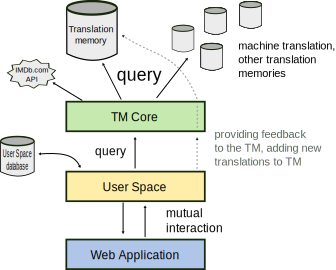
\includegraphics{figures/scheme.pdf}
\end{center}
\caption{Scheme of the application architecture.}\label{projectStructure:layers}
\end{figure}

The deepest level of the application is the Translation Memory Core which operates directly with the parallel chunks stored in database. It is implemented in Scala. It provides an interface for retrieving translation suggestions from multiple sources -- different ways of processing our own translation memory, publicly available translation memories or a machine translation output. It also assigns a score for each suggestion based on the retrieval parameters (typically the match score) and movie characteristics taken from the IMDb.com API.

The middle-ware layer is called the User Space (US). Its task is to interact with the translation memory itself and mirror all GUI operations on the server side. The User Space is implemented in Java. The TM Core is used only as a service which is queried for translation suggestions. The interaction with the GUI is much more complicated because each operation from GUI has to be reflected in the US. The US provides a permanent storage of users' work to make the whole application including the users data available from the Internet. Except this function, the US provides the TM suggestion for the GUI and keep them up to date (the TM is gradually improving, so after a week pause in work and a subtitle file, some better sentences in TM may occur).

GUI is written in Java, using GWT, which translates Java code into JavaScript and provides a framework for simple implementation of remote procedure calls (RPCs) through HTTP protocol, using POST requests. Server side of GUI layer displays the needed javascript and css code to user's browser, which, then, communicates with userspace through javascript AJAX calls through RPC, as described above. The GUI let the user log in, upload the subtitles, parses the subtitles to chunks, offer the user translations for every chunk and play the video of the chunks being translated.

Translation memory core and userspace are both parts of the same \texttt{.jar} file and are, therefore, run in the same java process. Userspace is running as a java servlet, because it is replying to RPC, which are implemented using HTTP post requests.

Server-side of GUI, which returns the HTML, CSS and JavaScript, is also in the same \texttt{.jar} file, together with needed GWT assets, and is run as a second servlet.

Both servlets are loaded using jetty webserver. Maven is used for building the application and retrieving dependencies, the Jenkins tool was used for continual building and testing of the project.

\section{Logical structure of work with TM}
\label{sec:shared_structure}

In this section, the general structure of work with translation memory is described, from which a design of common classes is inferred, later used both in US, GUI and Core.

\subsection*{User}
Everyone, who logs into the system, is called \emph{user}. Each user of the TM, except its own setting, authentication data etc., can own multiple subtitle files which we call \emph{Documents}.

\subsection*{Document}
\emph{Document} is subtitle file, owned by a user. (This is not connected with files, that are used for building the corpus.) The documents contains information about \emph{media source} of the subtitle, and list of the subtitles \emph{chunks} which either have been already translated or are waiting for translation.

\subsection*{Media source}
\emph{Media source} is our name for movie or TV show episode.

\subsection*{Chunk}
Chunk is our name for a piece of text, that is getting translated. Chunk has a \emph{surface form} -- the text, being translated -- plus possible annotations. One of the annotations are named entities, but we also save newlines and dialogue marks ("-") as an annotation, so it doesn't go into database.

We talk more about the nature of subtitle files in the part \label{subtitle_formats}.

\subsection*{Timed chunk}
Timed chunk is a chunk, that also have a time information and information about order, in which it appears in subtitle file.

\subsection*{Translation result}
The chunks are wrapped in to the \emph{Translation result} objects which contains the the timed chunk from the original subtitle file, a chunk produced by the user as a translation of the original chunk, a list of translation suggestions from translation memory \todo{Which are in fact WHAT? :)}which are in fact.


\begin{figure}[h]
\begin{center}
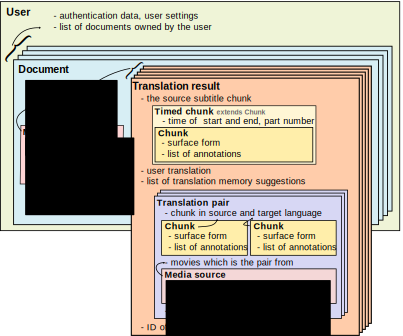
\includegraphics{figures/shared_classes.pdf}
\end{center}
\caption{Scheme of the application architecture.}\label{projectStructure:logical}
\end{figure}

All mentioned characteristics are common for both US and GUI. Because all parts of the project are Java based we can use a set of shared classes. Despite the limitations from to the fact, that the GWT implements only a subset of Java functionality, using a shared classes structure makes the whole project clearer. 

\subsection*{Annotations}

TODO \todo{Write something about the annotations}

%If we look at the structure of a document being translated which is mirrored in the GUI and in the US, we can notice there together parts originating in different part of the projects.

\section{Sharing the Implementation among the Project}

Since we are using Google Web Toolkit (GWT), we can share java classes between GUI and server, as described in \todo{where}??.

However, as noted in GWT documentation \footnote{\url{https://developers.google.com/web-toolkit/doc/latest/DevGuideCodingBasicsCompatibility} and \url{https://developers.google.com/web-toolkit/doc/latest/RefJreEmulation}}, not all java classes are directly translatable to GWT. The main issues are:

\begin{itemize}
\item the shared classes cannot reference any class, that is not translatable to JavaScript through GWT (for example, any third-party libraries)
\item the shared classes can use only a subset of Java runtime library. In our case, main case of this was \texttt{java.util.regex}, which is not implemented in GWT; we had to use \texttt{com.google.gwt.regexp.shared} instead
\item serialization works differently in GWT. What this effectively meant for us is that, even when we use general \texttt{List} interface for some property, we cannot set it as subtype of \texttt{List} that is not implemented in GWT (more concretely -- we wanted to use \texttt{scala.collection.JavaConverters.AsJava[List]} for scala $\Leftrightarrow$ java conversion)
\end{itemize}

Therefore, shared classes could only use a subset of Java (generally, what is translatable with GWT to JavaScript is also translatable by java compiler to JVM bytecode, but not the other way around).

\section{Usage of Third Party Libraries}

TODO \todo{write it, commented out pom file si right after this note}

%<dependency>
%        <groupId>org.hibernate</groupId>
%            <artifactId>hibernate-validator-annotation-processor</artifactId>
%            <version>4.1.0.Final</version>
%        </dependency>
%
%        <dependency>
%            <groupId>junit</groupId>
%            <artifactId>junit</artifactId>
%            <version>4.10</version>
%        </dependency>
%
%        <dependency>
%            <groupId>com.cybozu.labs</groupId>
%            <artifactId>langdetect</artifactId>
%            <version>1.1-20120112</version>
%        </dependency>
%
%            
%
%        <dependency>
%            <groupId>org.apache.xmlrpc</groupId>
%            <artifactId>xmlrpc-client</artifactId>
%            <version>3.1.3</version>
%        </dependency>
%
%                
%
%        <dependency>
%            <groupId>org.openid4java</groupId>
%            <artifactId>openid4java</artifactId>
%            <version>0.9.4.339</version>
%
%    </dependency>
%
%                        
%        <!-- for RPC -->
%        <!--<dependency>
%            <groupId>javax.validation</groupId>
%            <artifactId>validation-api</artifactId>
%            <version>1.0.0.GA</version>
%            <scope>test</scope>
%        </dependency>-->
%
%        <dependency>
%            <groupId>org.apache.commons</groupId>
%            <artifactId>commons-lang3</artifactId>
%            <version>3.1</version>
%        </dependency>
%
%        <dependency>
%            <groupId>org.apache.commons</groupId>
%            <artifactId>commons-math</artifactId>
%            <version>2.0</version>
%        </dependency>
%
%
%        <dependency>
%            <groupId>org.apache.opennlp</groupId>
%            <artifactId>opennlp-tools</artifactId>
%            <version>1.5.2-incubating</version>
%        </dependency>
%
%        <dependency>
%            <groupId>com.google.guava</groupId>
%            <artifactId>guava</artifactId>
%            <version>11.0.2</version>
%        </dependency>
%
%        <dependency>
%            <groupId>org.hsqldb</groupId>
%            <artifactId>hsqldb</artifactId>
%            <version>2.2.8</version>
%        </dependency>
%
%        <dependency>
%            <groupId>net.sf.trove4j</groupId>
%            <artifactId>trove4j</artifactId>
%            <version>3.0.2</version>
%        </dependency>
%
%        <dependency>
%            <groupId>org.eclipse.jetty</groupId>
%            <artifactId>jetty-webapp</artifactId>
%            <version>${jettyVersion}</version>
%        </dependency>
%
%        <dependency>
%            <groupId>org.eclipse.jetty</groupId>
%            <artifactId>jetty-jsp-2.1</artifactId>
%            <version>${jettyVersion}</version>
%        </dependency>
%
%        <dependency>
%            <groupId>org.eclipse.jetty</groupId>
%            <artifactId>jetty-server</artifactId>
%            <version>${jettyVersion}</version>
%        </dependency>
%
%        <dependency>
%            <groupId>org.scala-lang</groupId>
%            <artifactId>scala-compiler</artifactId>
%            <version>${scala.compiler.version}</version>
%            <scope>provided</scope>
%        </dependency>
%
%        <dependency>
%            <groupId>org.scala-lang</groupId>
%            <artifactId>scala-library</artifactId>
%            <version>${scala.compiler.version}</version>
%        </dependency>
%
%        <dependency>
%            <groupId>postgresql</groupId>
%            <artifactId>postgresql</artifactId>
%            <version>9.1-901.jdbc4</version>
%        </dependency>
%
%        <dependency>
%            <groupId>org.json</groupId>
%            <artifactId>json</artifactId>
%            <version>20090211</version>
%        </dependency>
%
%         <dependency>
%            <groupId>log4j</groupId>
%            <artifactId>log4j</artifactId>
%            <version>1.2.16</version>
%        </dependency>
%
%        <dependency>
%            <groupId>org.slf4j</groupId>
%            <artifactId>slf4j-api</artifactId>
%            <version>1.6.4</version>
%        </dependency>
%
%        <dependency>
%        	<groupId>org.slf4j</groupId>
%        	<artifactId>slf4j-log4j12</artifactId>
%        	<version>1.6.4</version>
%        </dependency>
%
%        <dependency>
%            <groupId>org.scalatest</groupId>
%            <artifactId>scalatest_2.9.0</artifactId>
%            <version>1.6.1</version>
%            <scope>test</scope>
%        </dependency>
%
%        <dependency>
%            <groupId>org.hibernate</groupId>
%            <artifactId>hibernate-core</artifactId>
%            <version>4.1.0.Final</version>
%        </dependency>
%
%        <dependency>
%            <groupId>com.google.gwt</groupId>
%            <artifactId>gwt-user</artifactId>
%            <version>${gwtVersion}</version>
%            <scope>provided</scope>
%        </dependency>
%
%        <dependency>
%            <groupId>com.google.gwt</groupId>
%            <artifactId>gwt-servlet</artifactId>
%            <version>${gwtVersion}</version>
%            <scope>runtime</scope>
%        </dependency>
%
%        <dependency>
%            <groupId>com.typesafe.akka</groupId>
%            <artifactId>akka-actor</artifactId>
%            <version>2.0.1</version>
%        </dependency>
%
%        <dependency>
%            <groupId>org.expressme</groupId>
%            <artifactId>JOpenId</artifactId>
%            <version>1.08</version>
%        </dependency>
%
%        <dependency>
%            <groupId>de.sven-jacobs</groupId>
%            <artifactId>loremipsum</artifactId>
%            <version>1.0</version>
%            <scope>test</scope>
%        </dependency>
%
%        <dependency>
%        	<groupId>net.liftweb</groupId>
%        	<artifactId>lift-json_2.9.1</artifactId>
%        	<version>2.4</version>
%        </dependency>
%
%        <dependency>
%        	<groupId>nz.ac.waikato.cms.weka</groupId>
%        	<artifactId>weka-stable</artifactId>
%        	<version>3.6.7</version>
%        </dependency>
%
%        <dependency>
%            <groupId>commons-validator</groupId>
%            <artifactId>commons-validator</artifactId>
%            <version>1.3.1</version>
%        </dependency>
%
%
%  <!-- Java Mail API -->
%	<dependency>
%		<groupId>javax.mail</groupId>
%		<artifactId>mail</artifactId>
%		<version>1.4.3</version>
%	</dependency>
%



%\chapter{Shared classes}
%

These classes can be shared by all parts of the project, but some of them are used only e.g. in GUI and Userspace.
\section{List of classes}
\todo{I would personally delete this}
annotations.gwt.xml \\
AuthenticationServiceType.java \\
Chunk.java \\
Document.java \\
DocumentResponse.java \\
FilmTitServiceAsync.java \\
FilmTitService.java \\
Language.java \\
MediaSource.java \\
TimedChunk.java \\
TitChunkSeparator.java \\
TranslationPair.java \\
TranslationResult.java \\
TranslationSource.java \\
User.java \\

./annotations: \\
Annotation.java \\
AnnotationType.java \\

./exceptions: \\
DatabaseException.java \\
InvalidChunkIdException.java \\
InvalidDocumentIdException.java \\
InvalidSessionIdException.java \\

./parsing: \\
Parser.java \\
ParserSrt.java \\
ParserSub.java \\
UnprocessedChunk.java \\

./tokenizers: \\
CzechSentenceTokenizer.java \\
EnglishSentenceTokenizer.java \\
SentenceTokenizer.java \\


\chapter{Building the Corpus}
\section{Initial data processing}

To ensure the full usability of the software from the very first moments when it is launched, some initial data is necessary.

\subsection{Retrieving data}

There are plenty of subtitle files in many languages available at the Internet these days, which can be easily downloaded.
However, it is problematic to download from most of the servers in bigger batches (thanks to anti-spam protection and so on); also, we wanted to avoid any copyright problems we would meet by using random subtitles from the internet. For this purpose, we asked the administrator of the biggest server providing the subtitles \emph{opensubtitles.org} for the data.

As a result of this we received all subtitle files in Czech and English from \emph{opensubtitles.org} with following licence condition (in Slovak):

\begin{quote}
\begin{verbatim}
Titulky mozem poskytnut, s tym ze:

- nebudu sa dalej sirit
- vsade, kde je to mozne a suvisi to s projektom, bude uvedena linka na
    www.opensubtitles.org (stranka programu, dokumentacia, program...)

Co sa tyka autorskych prav, tak neviem presne ako to je, ale myslim,
ze to je +- ok :)
\end{verbatim}
\end{quote}

\noindent with following English translation:

\begin{quote}
\begin{verbatim}
We can provide the subtitle files under following conditions:

- they won't be provided any further
- a link to www.opensubtitles.org will be placed whenever it's possible 
   (web page of the program, documentation, program itself...)

Considering the copyright law, I am not really sure how it is, 
but I think it's ok :)
\end{verbatim}
\end{quote}


\noindent We decided that this licence condition is acceptable for our purposes. 

As a matter of fact, the users of \emph{opensubtitles.org} agree with a statement where they declare they are holders of all rights to the content they post to the server, and provide the subtitle files as their own intellectual property for public use. Based on this and the licence, we think there are no more copyright issues.% Based on this statement we trust the users they really did what they declared.

%From this data we will create a parallel corpus of ...

\subsection{The data properties}

(In this section, we call \emph{subtitle} the whole subtitle file, \emph{chunk} is again the piece of text, displayed on screen at one time)

We received 3,076 MB of data in 139,538 files with a database index dump which did not exactly match the received content. After solving this problem we have 39,712 Czech subtitle files and 97,991 English files of 15,881 movies or TV shows episodes -- 3,032 MB of data.


Some subtitles are divide into more files, anyway 81\% of subtitles are in one piece. There is also just 1.7\% movies having subtitles only in multiple files. Moreover, we can assume that those which are in more parts, are probably just split the complete onces. To keep the chunk alignment simple we would delete those as well.

This caused that some movies lost its translation -- 64
of Czech and 218 of English. In total we will lost 3,5\% of movies. After this steps, the amount of data was 2,556 MB.

Because OpenSubtitles internally uses IMDB for adding information about movies and TV shows to subtitles, it was not hard to align subtitles of same movies and TV show episodes together, since all movie names used the same format (name and year), and the TV episodes were correctly marked.

However, this also caused one curious issue.
While looking more carefully at the data, we found there were 228 Czech subtitles files, 814 files in total having one particular movie ID and containing various content. This movie was Carmentica, a 21 seconds long silent film from 1884. This happened due to a server error at \emph{opensubtitles.org}, because the movie has ID {\tt tt0000001} at IMDB.

After doing all mentioned filtering we had 2,543 MB in 110,312 subtitle files (32,705 Czech, 77,607 English) of 15,552 movies / TV shows' episodes.

From these, the average subtitle file had XX chunks.

\subsection{Aligning the subtitles}

While we had enough metadata to align subtitles of the same movie together, there were still more than two subtitle files for each of the movies, so we needed to chose the best pair. Also, on these, we needed to align the actual chunks together. 

For elignment, we used two different approaches, which we then compared. TODO: COMPARISON. Damn, I am doing that today.

\subsubsection*{Editing distance}

While comparing two mostly identical subtitle files, there may appear some issues which cause that the timing of the files is not identical. There exist some cases where one chunk is split into more or two are merged into one. In both of this cases, two time declarations in the file remain the same and two time declarations are added or deleted. There are also a lot of subtitles for deaf people where from time to time some additional subtitle appears. 

From that we concluded that the best measure how subtitle files matches would be the editing distance of their time declarations since the cases mentioned above contributes relatively little to the score in contrast to some more significant mismatches. 
By that we mean taking all the time information (both the starts and the ends) as vectors, and then counting editing distance of those two vectors by dynamic algorithm.

As one of the papers (CITE!!!) proposed we used 0.6\,s as a tolerance for equality, not to be confused by slight differences in timing. Because the computation on whole files would be really time consuming, we limited it just for the first 100 time declarations in the files.

%when I rewrote it to scala it was actually much faster then in perl. Maybe we COULD do the whole files now :-)

The results were following: from 15,552 movies there was 22.2\,\%
with perfect matches and 3.1\,\% of total mismatches. The scores for partial matches are captured in table \ref{opensubtitles:matchTable}.

\begin{table}[h]

\begin{center}
\begin{tabular}{|c|c|}
\hline
amount of films & measure of match\\ \hline
22,2 \% & $= 100 \%$ match \\
45.7 \% & $\ge 90 \%$ match \\ 
56.2 \% & $\ge 80 \%$ match \\ 
63.0 \% & $\ge 70 \%$ match \\
69.2 \% & $\ge 60 \%$ match \\ \hline
\end{tabular}
\end{center}

\caption{Table capturing for how many movies there exist a matching pair of subtitle files with given measure of matching}\label{opensubtitles:matchTable}
\end{table}

%what does the "measure of match" mean in this context? I don't get it.

After looking at some randomly selected files we have decided to use just movies for which we have a pair of files with at least 70 \% match. Surprisingly, some worse scored pairs have quite high-quality translations, because they contain a lot of joined and split chunks, but generally, based on ran the quality of translation decreased with the match score.

On this files we run an aligning algorithm based just on the timing. The chunks were aligned if both the time of their start and time of their end differ less than by 0.6\ s. This gave us 884 MB of parallel data which consists of 13,636,022 chunks. In this we have 5,669,837 unique chunks, from which 3.7 \% appears more than once. On the other hand, chunks appearing more than once make 57.6 \% of the whole corpus.


\chapter{Core Translation Memory}
This chapter describes the design and implementation of the core translation memory. The core translation memory is the part of the project that is responsible for retrieving and ranking suitable suggestions for chunks in the subtitle file that the user is translating.

\section{Preliminaries}

\subsection{Choosing a DBMS}
\label{sec:dbms}

For the choice of a suitable database management system underlying the
core translation memory and the user space, the main points we
considered were

\begin{itemize}
\item
  software license of the DBMS
\item
  general performance and maintainability
\item
  included support for fuzzy matching and custom indexes
\end{itemize}
According to these requirements, we evaluated several database systems
and selected the open source database system
\postgres.\footnote{\url{http://www.postgresql.org/}, written either Postgres or PostgreSQL} This system
fulfills the requirements as follows:

\begin{itemize}
\item
  open license similar to BSD license
\item
  good results in performance evaluations and good reputation for
  maintainability
\item
  support for phonetic representation of strings (SOUNDEX and
  METAPHONE), string edit distance (Levenshtein), fuzzy string search
  using character trigrams and customizable indexes (GIST, GIN)
\end{itemize}

For managing connections to the database in Java and Scala, we use JDBC, 
which allows the database connection to easily use another DBMS. 
In the XML-based configuration file (see the installation manual, Chapter~\ref{chap:technical_manual}), the JDBC connector
and username and password to the database have to be specified. When testing the
translation memory with project-internal unit tests, we replace the production JDBC
configuration with a temporary in-memory database (HSQLDB\footnote{\url{http://hsqldb.org/}}).

\lstset{language=XML, caption={Configuration snippet}}
\begin{lstlisting}
<database>
    <connector>jdbc:postgresql://localhost/filmtit</connector>
    <user>postgres</user>
    <password>postgres</password>
</database>
\end{lstlisting}


\subsection{Retrieving Media Source information}

For retrieving information about media sources, we initially used a free IMDB API (\url{http://imdbapi.com/}). However, it showed that this API might become unreliable in the future and indeed, as of July 30, the API had been shut down. To avoid complications early, we switched to the Freebase API\footnote{\url{http://www.freebase.com/}}. Freebase is a large knowledge base of structured data based on data extracted from Wikipedia and other publicly available resources and continually extended by users.

To retrieve media source candidates, first a full text search query with the title and a restriction to entities of type \emph{film}\footnote{Freebase type: /film/film.} and \emph{TV program}\footnote{Freebase type: /tv/tv\_program.} is sent to the Freebase API. Afterwards additional information for each candidate is retrieved and the {\tt MediaSource} objects are sent to the GUI for the best match to be selected by the user.



\section{Architecture of the Core Translation Memory}
\label{sec:corearchitecture}

The core translation memory consists of the database of chunks and media
sources (movies and TV shows) which are indexed in several ways for fast
retrieval. A query to the translation memory generally proceeds in two
steps: In a first step, translation pairs for a chunk are retrieved from
the database. The second step consists of ranking the candidates
retrieved in the first step according to their quality and how well they
match the query. If the quality of the retrieved candidates exceeds a
minimum quality threshold, they will be sent to the user.

\subsection{Backoff translation memories}

The idea of a backoff translation memory is to use multiple ways of
retrieving and ranking candidate translation pairs from the database and
``back off'' to a less exact level of retrieval and ranking when there
are no satisfying results on the current level.

A backoff-level in the translation memory consists of a \emph{translation pair
searcher}, a \emph{translation pair ranker} and a \emph{minimal quality
threshold}. 
If the results retrieved by the \emph{searcher} and scored and ranked by
the \emph{ranker} do not meet the threshold, then the query is sent to the 
next level of the backoff translation memory. 


\section{Candidate retrieval}
\label{sec:candidate_retrieval}

We implemented several methods for efficiently retrieving candidate
translation pairs from the database. 


\subsection{Translation pair searchers}

Every translation pair searcher implements the interface {\tt TranslationPairSearcher} and therefore must implement the method 

\vspace*{0.5em}

\lstset{language=scala, caption={Candidate search}}
\begin{lstlisting}
def candidates(chunk: Chunk, language: Language): List[TranslationPair]
\end{lstlisting}

This is the main method for retrieving translations pairs, which are then combined and ranked in later steps. A {\tt TranslationPairSearcher} may require the chunks it queries to be tokenized beforehand. In this case, the {\tt TranslationPairSearcher} must override the following method:

\vspace*{0.5em}

\lstset{language=scala, caption={TranslationPairSearchers may require tokenization}}
\begin{lstlisting}
def requiresTokenization: Boolean
\end{lstlisting}

\vspace*{0.5em}



{\tt TranslationPairSearcher}s that are based on the local \postgres~database extend the class {\tt TranslationPairStorage} and must implement the method {\tt add} for adding new translation pairs to the storage.

\vspace*{0.5em}
 
\lstset{language=scala, caption={TranslationPairSearchers may require tokenization}}
\begin{lstlisting}
def add(translationPairs: TraversableOnce[TranslationPair])
\end{lstlisting}

\vspace*{0.5em}


The method {\tt reindex} must be implemented to create and update the database indexes for the particular searcher.

\lstset{language=scala, caption={TranslationPairSearchers may require tokenization}}
\begin{lstlisting}
def reindex()
\end{lstlisting}








\subsection{Tokenization}
\label{sec:tokenization}

For all program-based retrieval methods, we tokenize, i.e.\ separate the input sentence into individual tokens,
all inputs, using tokenizers provided by the Apache OpenNLP project.\footnote{\url{http://opennlp.apache.org/}}
OpenNLP provides both unsupervised and supervised methods of tokenization. 
As a default tokenizer, we use an unsupervised tokenizer that splits the input
based on whitespace. This method has the advantage that it is applicable to any new
language without requiring further training, however the result is of moderate
quality and often leads to problems in latter processing steps (e.g. Named Entity Recognition).

To improve the results, we use a Maximum-Entropy based OpenNLP tokenizer. For English, we use the
models provided by the OpenNLP project. 


\subsubsection*{Czech ME tokenizer}

For Czech, no such model existed, so we trained a ME tokenizer
model on data from the Prague Dependency Treebank\footnote{\url{http://ufal.mff.cuni.cz/pdt2.0/}}. Scheme of the process is in fogure \ref{fig:tokenizer}. 

We produced a script that creates training data in the following format:
\begin{verbatim}
K vynikajícím spisovatelům<SPLIT>, kteří věřili v nevysvětlitelné duševní 
úkazy<SPLIT>, patřil také americký romanopisec Upton Sinclair<SPLIT>.
\end{verbatim}

\begin{figure}[h]
\begin{center}
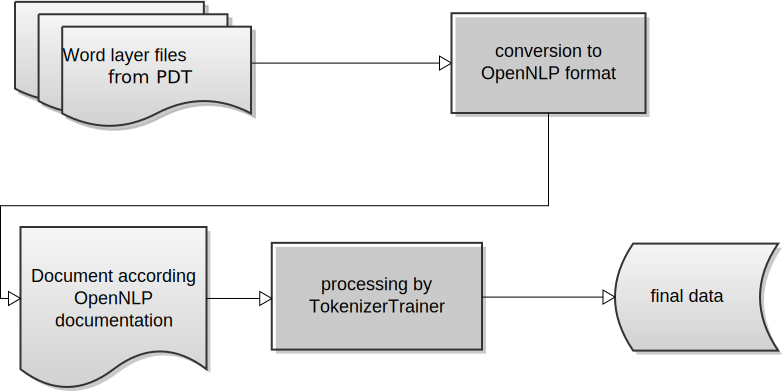
\includegraphics[scale=0.6]{figures/creatingTokenizationModel.pdf}
\end{center}
\caption{Scheme of traning the tokenizer.}
\label{fig:tokenizer}
\end{figure}

In the training data, the \verb|<SPLIT>| annotation indicates a position in the data, in which the
tokenizer is required to separate two tokens (in this case words and punctuation symbols). These
positions were manually marked in the Prague Dependency Treebank by annotators.

On a test dataset from the Prague Dependency Treebank, the ME tokenizer achieved the following results:

\lstset{caption={Accuracy for the Czech ME tokenizer.}}
\begin{lstlisting}
Precision: 0.9970180340649772
Recall: 0.9954658318039512
F-Measure: 0.9962413283293529
\end{lstlisting}


\subsection{Signature-based retrieval}


The most general method is the usage of indexed signature strings. There are two implementations of signature-based retrieval in the project: In the first method, signatures are created fully within the \postgres~database (database-based signatures) and in the second, the signatures are created on the server and only stored and retrieved in the
database (program-based signatures).  


\subsubsection*{Program-based signatures}

In the case of program-based signatures, for each chunk stored in the database, a string is produced by a signature function and this string is used to retrieve candidates from a signature table that is in turn
connected to the translation pairs table.

\begin{figure}[h!]
	\centering
		\includegraphics[width=17cm]{figures/core/signatures.pdf}
	\caption{Illustration of signature strings in the database.}
	\label{fig:figures_core_signatures}
\end{figure}


\subsubsection*{Database-based signatures}

In the case of the database-based signatures, a {\tt PL/pgSQL} procedural function is used to create a functional index\footnote{See e.g.\ \url{http://www.postgresql.org/docs/9.1/static/indexes-expressional.html} (retrieved 02.08.2012).} on the translationpairs table. The function can then be used for fast retrieval from this table.


Several signature functions are used in the translation memory
implementation. In the following sections, the signature functions and related issues will be illustrated.


\subsection{Signature-based retrieval: Exact matches}

The first signature function is for retrieving exact matches. For this,
the signature function consists of the first letters of each word in the
chunk. Punctuation is dropped from the signature. If the queried chunk is
short, only using the first letter would produce a very high number of
results. Hence, for short chunks, more letters of each individual token are
included. Algorithm~\ref{alg:firstletter} shows pseudo-code for the {\tt FirstLetter}
function.

\vspace{1em}
\begin{algorithm}[H]
\label{alg:firstletter}
 \SetKwFunction{Union}{Union}\SetKwFunction{TokenizeAndRemoveStopWords}{TokenizeAndRemoveStopWords}
 \SetKwFunction{Union}{Union}\SetKwFunction{Lower}{Lower}
 \SetKwFunction{Union}{Union}\SetKwFunction{Take}{Take}


 \SetAlgoLined

 \KwData{text chunk}
 \KwResult{signature for the chunk}
 $tokens \leftarrow \TokenizeAndRemoveStopWords{chunk}$

 \For{$token \in tokens$}{

   \uIf{$|token| = 1$}{
     ret += \Lower{token}
   } \uElseIf{$|token| = 2$}{
     ret += \Lower{\Take{3, token}}
   } \uElseIf{$|token| = 3$}{
     ret += \Lower{\Take{2, token}}
   } \Else{
     ret += \Lower{\Take{1, token}}
  }

 }
 \Return ret joined by " "
 \caption{{\tt FirstLetter} function.}
\end{algorithm}





\subsection{Signature-based retrieval: Named Entities}

The second, more fuzzy signature function uses named entity recognition
to provide matches. Named entity recognition is the task of finding
elements in a text belonging to basic name categories like
\emph{Person}, \emph{Organization} and \emph{Place}. In the signature,
the surface form of the named entity is replaced by its named entity
category. This allows the retrieval of candidate chunks that differ only
in the named entities they are using. As an example, consider the
following chunks:

\lstset{caption={Example of NE-based retrieval.}}
\begin{lstlisting}
Chunk 1:   Peter saw the girl.
Signature: <Person> saw the girl

Chunk 2:   Thomas saw the girl.
Signature: <Person> saw the girl
\end{lstlisting}

Using the named entity-based signature, Chunk 2 can be retrieved as a
candidate for chunk 1. Since an exact match would be preferable, this 
will only be used if there is no better fitting candidate in the
database.

\subsubsection{Named Entity Recognizers}

For Named entity recognition, we use the OpenNLP Maximum Entropy based
Named entity recognizers. For English, we were able to use the pre-trained
models for persons, organizations and places that are available through the
OpenNLP project.

For Czech, no such models were available, hence we trained our own models based
on various data sources and then chose the best models from the comparison 
of two approaches of acquiring training data.


\subsubsection*{First approach: Training data based on Wikipedia and DBpedia}

Our first approach to acquiring named entity recognition training data for Czech 
was based on the Pig NLProc utility\footnote{\url{https://github.com/ogrisel/pignlproc}}.
Pig is an Apache project providing platform that features a SQL-like syntax
for data analysis based on Apache Hadoop. The Pig NLProc utility provides a number
of Pig scripts to extract natural language processing training data from Wikipedia
and DBpedia.

DBpedia is a \footnote{\url{http://dbpedia.org/About}} community project for extracting 
structured data from Wikipedia. Based on user-created mappings of Wikipedia info boxes to
an ontology, DBpedia provides data that allows to easily select DBpedia entites that 
correspond to persons, organizations, places, etc.

To acquire named entity recognition training data, the Pig NLProc utility searches
for article references to Wikipedia pages that are known (from the DBpedia ontology)
to be of the required types (e.g. Person). These instances are sentences with links
to the given article and these are then converted to the training format required 
by OpenNLP.

For Czech, user-generated mappings for many info boxes are already available, however,
the DBpedia data for Czech is not yet available. Hence, we downloaded the DBpedia
extraction framework with the Czech data and ran the extraction process ourselves.
With the resulting data and the Pig NLProc scripts (which required minimal changes
for issues of compatibility), we produced training data for named entities of the types
Person, Place and Organization.



\subsubsection*{Second approach: Training data based on the Czech Named Entity Corpus}

The second approach is based on the Czech Named Entity corpus.\footnote{\url{http://ufal.mff.cuni.cz/tectomt/releases/czech_named_entity_corpus_10/index.html}}
The corpus contains manual named entity annotations of a large number of named entity types. Figure~\ref{fig:figures_core_CzechNECorpus}
shows an overview of the NE types annotated in the corpus.


\begin{figure}[h]
	\centering
		\includegraphics[width=10.5cm]{figures/core/CzechNECorpus.pdf}
	\caption{Named entity types in the Czech Named Entity corpus. Source: Czech Named Entity corpus documentation.}
	\label{fig:figures_core_CzechNECorpus}
\end{figure}


We wrote scripts that convert the XML-based format of the corpus to the format required by OpenNLP, 
manually selected the annotation types and trained the OpenNLP named entity recognizers on the resulting data.


\subsubsection*{Selecting the best approach}

Both approaches showed to have their unique advantages and disadvantages. While the first approach is 
only minimally supervised and can easily be extended to other languages that have a local version of 
Wikipedia and existing DBpedia dumps (DBpedia dumps are currently available for 97 languages\footnote{\url{http://wiki.dbpedia.org/Downloads37}}), 
our manual evaluation of the produced Named Entity recognizers showed that the 
models trained on the Czech Named Entity corpus produced better results.

More precisely, we approximated, that the DBpedia recognized far less cases and, therefore, had much lower RECALL, the PRECISION was only slightly better. We then decided, that lower RECALL is worse for our purposes -- it is better to show wrong translation to user than to not show anything.

\subsubsection*{Effectiveness}
It is worth noting that the overall effectiveness of using named entity-based retrieval was worse than we anticipated. In most subtitles, there are only few matches, but the recognition of named entities takes the most time during the data import. For this reason, we kept NE-based retrieval as a retrieval level in the core, however, we are not currently using it since the other methods already provide reasonable results and are easier to adapt to new languages and faster.

\subsection{Full-text search}

As another, more fuzzy level of retrieval, we use the full-text search included in \postgres. In  \postgres~full-text search, documents (in our case translation pairs) are tokenized and normalized. The result of this process is vector of normalized tokens ({\tt tsvector}). The normalization step can include lowercasing, stemming or synonyms from a dictionary and removes stop words. \postgres~builds an index over the token vector of all documents, against which queries can be run. To convert a string to a query, it is tokenized and normalized and the resulting normalized tokens are connected with an {\tt AND} operator.

The tokenization and normalization for a specific language is described in a text search configuration.\footnote{\url{http://www.postgresql.org/docs/9.1/static/textsearch-intro.html}} By default, \postgres~includes text search configurations for the following languages: Danish, Dutch, English, Finnish, French, German, Hungarian, Italian, Norwegian, Portuguese, Romanian, Russian, Spanish, Swedish, Turkish and the default ``Simple'' configuration. For Czech, a text search configuration is available from postgres.cz\footnote{\url{http://postgres.cz/wiki/Instalace_PostgreSQL}} For installation instructions, please see the technical manual in chapter~\ref{chap:technical_manual}.

When querying candidates for a Chunk, we use the {\tt ts\_rank}\footnote{\url{http://www.postgresql.org/docs/9.1/static/functions-textsearch.html}} function to pre-sort the candidates and the {\tt ts\_rank} score is later used as one of the scores in the ranking of translation pair candidates. One problem that the full-text search as a method of candidate retrieval shows, is that some of the candidates are unreasonably large documents that still have high scores because their token overlaps with the query are reasonable. We approach this problem by using our own ranking functions for translation pairs, as described in Section~\ref{sec:ranking}.


\subsection{External services}

As another backoff level, we use Machine Translation from external services.
For this, a query with the chunk is sent to an external REST-based API. We offer a translation pair searcher for the free Machine Translation API of the MyMemory project.\footnote{ \url{http://mymemory.translated.net/doc/spec.php}} However, there is currently no machine translation service with an unlimited free API, and, for example, the MyMemory project has such a low daily quota (2500 requests/day) that the quota is quickly surpassed when translating subtitle files.

\subsection{Statistical Machine-Translation based on Moses}
\label{sec:statmtmoses}

We tried Machine Translation first as an experiment, but it turned out the results are very good and, after some optimizations, very fast.

Moses\footnote{\url{http://www.statmt.org/moses/}} is a very popular statistical machine translation system that can work both with phrase-based models (which we use) an tree-based models (which require grammatical annotations).

We run Moses as a separate process in server mode. The sentences are sent to the Moses server through Apache's XML RPC client\footnote{It is modeled after SampleClient in Moses, \url{https://github.com/moses-smt/mosesdecoder/blob/master/contrib/server/SampleClient.java}} sentence by sentence. We have to send the sentences to Moses server already tokenized and it produces better results if the first letters of sentences are lowercased.

Because we have limited computing resources, we trained only English to Czech machine translation, since that will be most used. If we wanted to train Czech to English too, used resources would double. More information about training the machine translation and getting it to work fast can be found in Chapter~\ref{chap:moses}.

The tokenization of the input sentences, however, turned out to be problematic. Because we did not see it as a problem (since tokenization does not seem like a big problem at the first glance), we just tokenize the input with the OpenNLP tokenizers and we let Moses use its own tokenizers.

Moses, however, tokenizes English slightly different. This causes problems with the contractions of English suffixes like \texttt{-n't} and \texttt{-'ll}. For example, we tokenize \texttt{don't} as \texttt{do n't}, Moses tokenizes it as \texttt{don 't}. Those are very widely used and their wrong tokenization will, of course, produce very wrong results.

For that reason, we had to add some corrections of tokenization for the contraction suffixes -- there are not that many of them, but they are so frequent and important that we had to fix it somehow. Those corrections are hardcoded in the \texttt{MosesSearcher.scala}. This is not an ideal solution (for example, it will break with addition of a new language); more optimal solution would be to use the same tokenizers in our application and in Moses training. However, we noticed it only later, when there was no time for correction on either our database or the Moses corpus.


\section{Candidate Ranking}
\label{sec:ranking}

After retrieving candidates for a query, the candidate translation pairs must be ranked according to their quality and how well they fit the queried chunk. We use different methods for ranking the candidates retrieved by the various candidate retrieval methods. In the following section, we will briefly describe the ranking methods for each retrieval method.

All ranking methods are based on a combination of scores. Depending on the retrieval method, we assign every translation pair candidate a set of scores, which are then combined into a final score. Translation pairs are ordered by this score.

To learn the best combination of scores, we manually selected translations for heldout subtitle files and then used those annotations as positive and negative examples for training a model using the WEKA machine learning toolkit.\footnote{\url{http://www.cs.waikato.ac.nz/ml/weka/}}

\subsection{Training the models}

For the manual annotation required to estimate weights for the scores, we started the translation memory with only the corresponding backoff level (e.g.\ exact matching or fuzzy matching) and translated heldout subtitle files using the translation workspace. After uploading and finishing the subtitle files, the class {\tt cz.filmtit.dataimport.training.GenerateTrainingset} can be used to generate a CSV file in WEKA-compatible format which can then be used to train a model.

For creating positive and negative instances, chunks without any suggestions from the translation memory are ignored. If a translation pair was selected, it is used as a positive example. If no translation pair was selected by the user, a random translation pair from the first ten suggestions is selected and used as a negative example. We select 


\subsection{Ranking for exact matches}

The ranking for exact matches uses a linear regression model with the following scores:

\begin{itemize}
	\item \textbf{translation pair count}\\
	The translation pair count specifies how often a translation pair has been observed. This score is calculated as $\frac{c(p)}{ \sum_{p' \in P}{c(p')}  } $\ , where $c(p)$ is the count for the translation pair $p$ and $P$ is the set of all translation pair candidates for a query.
	
	\item \textbf{source-chunk edit distance}\\
	The edit distance between the queried chunk and the source chunk of the translation pair candidate; the score is normalized by the length of the queried chunk.
	
	\item \textbf{genre match}\\
	Percentage indicting how much the genres of the queried media source overlap with the genres of the sources of the translation pair.

	\item \textbf{length difference between source and translation}\\
	The length difference between the source and target side of the translation pair candidate may indicate that an alignment is not of high quality (in most good translation pair candidates,  the length source and target side should not differ in length significantly).
	
	\item \textbf{final punctuation}\\
	Feature indicating whether the final punctuation of the queried chunk and the candidate translation match.
	
	
	
\end{itemize}



\subsection{Ranking for full-text search matches}



\begin{itemize}
	
	\item \textbf{full-text search score for the document}\\
	The score assigned by the \postgres~full text search for the document that represents the translation pair candidate.
    
	\item \textbf{translation pair count}\\
	The translation pair count specifies how often a translation pair has been observed. This score is calculated as $\frac{c(p)}{ \sum_{p' \in P}{c(p')}  } $\ , where $c(p)$ is the count for the translation pair $p$ and $P$ is the set of all translation pair candidates for a query.
	
	\item \textbf{source-chunk edit distance}\\
	The edit distance between the queried chunk and the source chunk of the translation pair candidate; the score is normalized by the length of the queried chunk.
	
	\item \textbf{genre match}\\
	Percentage indicting how much the genres of the queried media source overlap with the genres of the sources of the translation pair.

	\item \textbf{length difference between query and source}\\
	The length difference between the queried chunk and the source side of the translation pair candidate 


	\item \textbf{length difference between source and translation}\\
	The length difference between the source and target side of the translation pair candidate may indicate that an alignment is not of high quality (in most good translation pair candidates,  the length source and target side should not differ in length significantly).
	
	\item \textbf{final punctuation}\\
	Feature indicating whether the final punctuation of the queried chunk and the candidate translation match.

\end{itemize}



\section{Merging similar candidates}

After all translation pair candidates are retrieved and ranked on each level, we attempt to merge translation pairs that are too similar, so not to present the user with several choices that differ only very slightly.

As a translation pair merger, we currently use an implementation based on Levenshtein distance, which removes all candidates whose similarity to a higher-scoring candidate are below a given threshold (1 by default).

%TODO algorithm+analysis



\section{Technical issues}

\subsection{Concurrency}

One important issue in the Core Translation Memory is that the service must be able to handle a large number of simultaneous requests without blocking or long delays. There are, however, some searchers, that are inherently not thread-safe.

To approach this issue, we used the Scala akka library,\footnote{\url{http://akka.io/}} which provides methods for parallelization based on the \emph{actor model}. A {\tt TranslationPairSearcherWrapper}\footnote{See  the class cz.filmtit.core.concurrency.searcher.TranslationPairSearcherWrapper.} is a {\tt TranslationPairSearcher} that is constructed with a number of other {\tt TranslationPairSearcher}s, which act as the wrapper's workers. When the {\tt TranslationPairSearcherWrapper} receives a request, it routes it to a free worker or adds it to the queue if none of the workers are free. Using this wrapper class, any non-thread-safe subclass of {\tt TranslationPairSearcher} can easily be queried in parallel.

We use the same method for parallelizing the tokenization of Chunks, since it is not thread-safe either.


\subsection{Keeping the database up to date}

Since we want to ensure good retrieval performance, the core database is read-only in production mode. The user's translations that are stored in the User Space already are periodically added to the core database as new translation pairs and the indexes of all searchers are updated in turn.





\chapter{Training machine translation}
\label{chap:moses}

\todo{This whole chapter is VERY dense and VERY technical. I will have to rewrite it to something more readable..... MAYBE... DAMN THERE IS NO  TIME FOR ANYTHING}

Although our initial plan was to show translation memory only to the translator, we found out that we can also use the corpus to train a model for statistical machine translation. However, we also found that despite getting quite good results from the translation, the durations for getting the translations were too long, compared to the translation memory.

In this chapter, we will describe, how we trained the models, our results and how we managed to get the time cost down. The final model is a part of our project; the script to produce the model from the aligned data is not included, since it would require changes to EMS source code\footnote{EMS is the Experiment Management System, a system for managing Moses experiments, \url{http://www.statmt.org/moses/?n=FactoredTraining.EMS}}, which are untested at the moment and beyond the scope of this project.

Since we focus mainly on English to Czech translation, we modeled, trained and tested only for this way of translation. Training for the opposite way of translation would be possible, too, but all the necessary resources would double, while it would only benefit a small number of people.

This chapter requires some knowledge of phrase-based translation models and Moses in general. If you are not familiar with either, the short version of this chapter is that we are getting -- on subtitles -- better results with our machine translation than Google Translate, we are getting it fast, and we were able to fit it on a rather small virtual machine.


\section{Initial setup}
\subsection{Initial settings}

For training machine translation, we use our subtitle corpus, aligned by techniques described in Section~\ref{sec:aligning_subtitles}. Since we want to be more exact in this case, we used a more strict alignment, with 0.6\,s tolerance.

We do not require all the metadata about movie files for this task, so we added all the data together. We took away 15,000 sentences for MERT tuning (which proved to be too much) and 5,000 sentences for testing. The rest is training data.

Because of the way we took the testing sentences, they are all from different movies than the training data, except for at most one movie, that can have different sentences both in tuning and testing.

We run the standard EMS\footnote{EMS is the Experiment Management System, a system for managing Moses experiments, \url{http://www.statmt.org/moses/?n=FactoredTraining.EMS}} scenario on our data, which includes testing and counting BLEU score\footnote{BLEU is an automatic metric for measuring the success of a translation}. Although EMS counts both case-sensitive and case-insensitive BLEU, we chose the case-insensitive one.

We chose EMS instead of UFAL's own \texttt{eman}, simply for better documentation of the former and the inclusion of EMS in the standard Moses installation.

Initially, for the language model, we chose the IRSTLM\footnote{\url{http://hlt.fbk.eu/en/irstlm}} language model. For the translation model training, we used standard GIZA++.

We also measured the time for running the test translation.\footnote{This was achieved by adding time tracking code to the EMS source code; this code was submitted to Moses and actually ``survived'' in the main git repository for a few weeks, but was ultimately deleted, because it broke some edge cases.} Time was measured on a machine with Intel Core2 Quad CPU Q9550, with 4 cores with 2.83GHz, and 4GB of memory.

For reference on quality, we also translated the test set with Google Translate.

\begin{figure}[h]
\begin{center}
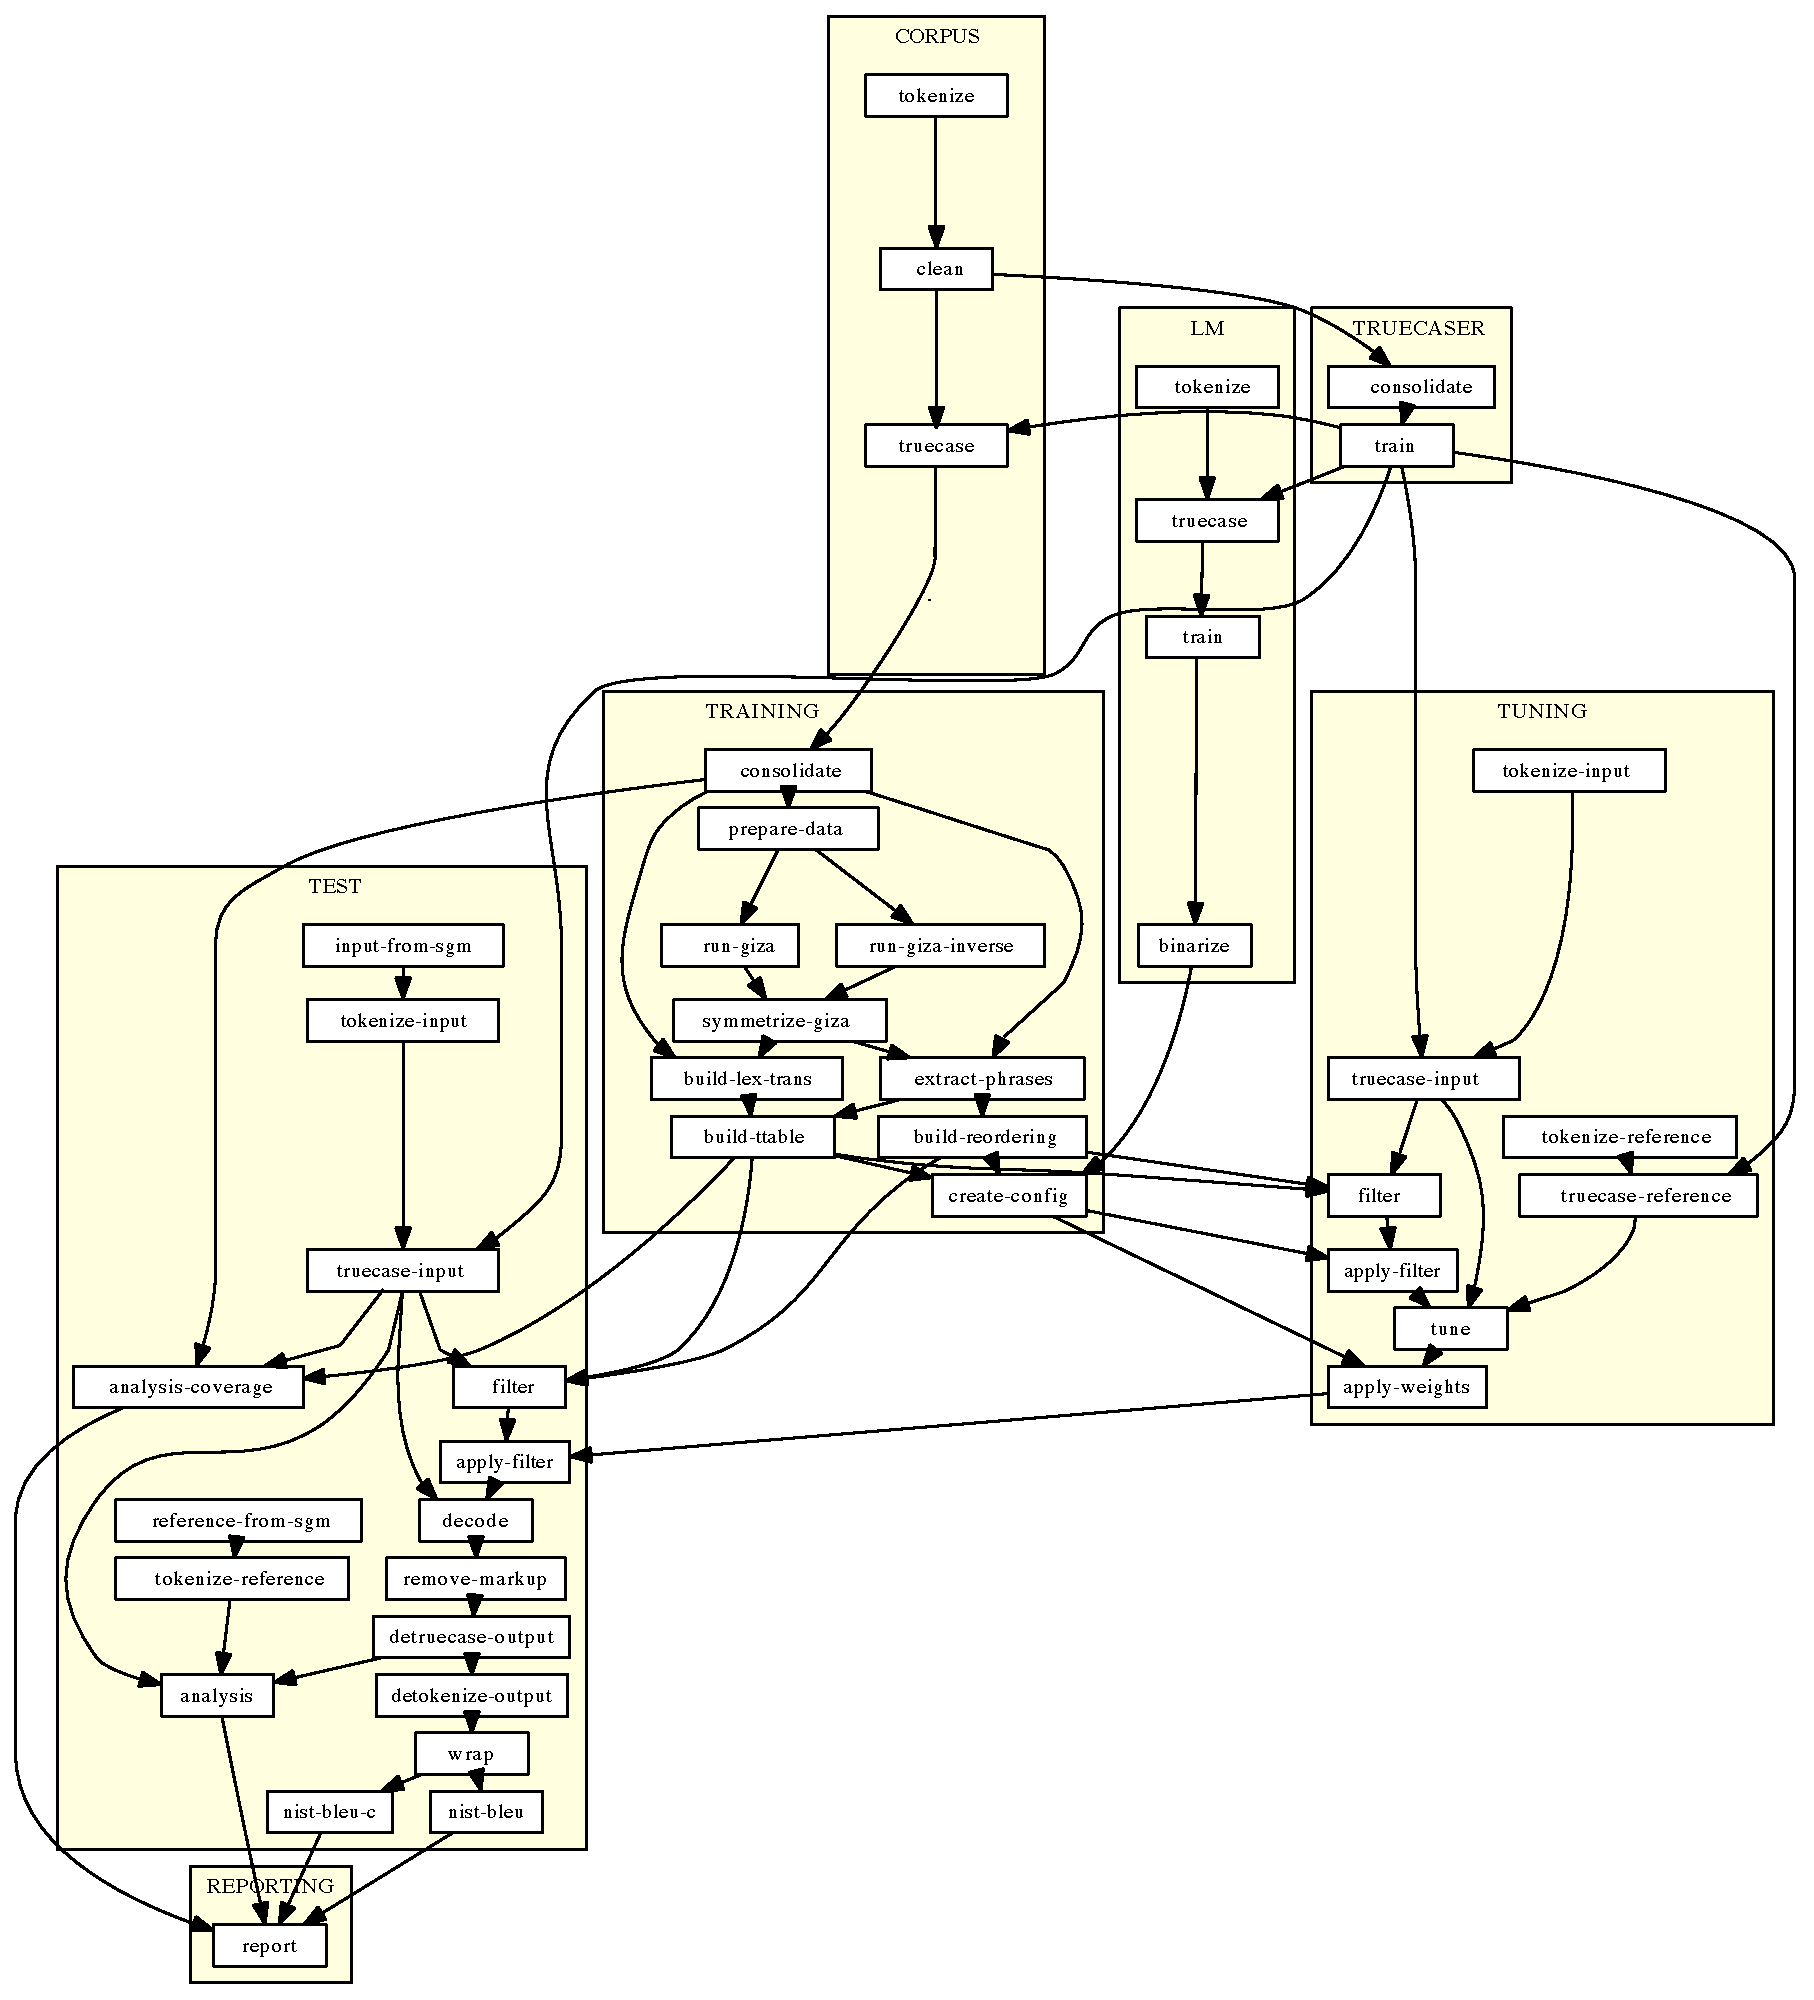
\includegraphics[width=0.8\textwidth]{figures/moses_13_graf.pdf}
\end{center}
\caption{Initial EMS set-up}\label{moses:initial}
\end{figure}

We can see the initial set-up in Figure~\ref{moses:initial}.
\subsection{Initial results}

The initial results are shown below.

\begin{table}[h]
\begin{center}
\begin{tabular}{|l|l|r|}
    \hline
    \textbf{Type} & \textbf{BLEU} & \textbf{incomplete average time per sentence} \\ \hline
    Initial setup & 23.88 & 147\,ms \\ \hline
    Google Translate & 19.07 & N/A \\  \hline
\end{tabular}
\end{center}

\caption{Initial results}\label{moses:initialresults}
\end{table}

We were very pleasantly surprised that our initial results were better than Google Translate, without really doing anything ``smart'' on our part. This is, however, definitely caused by a smaller domain. On the \texttt{newstest2012} set, Google's results were still quite good, while ours were terribly low\todo{I don't have time to show concrete numbers now. If I have more time, will do.}; the phrases in newspapers are completely different than phrases in subtitles.

The time looked good on the first glance; however, real times observed didn't line up with the results with the model. The difference was actually caused by EMT filtering (seen on \ref{moses:initial} as ``filter''). EMT, before doing the final tests, actually filters the models in such a way that only needed parts are loaded; the actual time of the final test is, then, much lower.

Also, even when we did not optimize for time spent on initial learning, the learning phase was too long to make any experiments effective. We addressed this issue, too.

\section{Changes in the set-up}
\subsection{Tuning set size}
The biggest issue with the training was actually the MERT tuning. If we cut down the number of phrases for MERT tuning, the time for tuning decreases significantly, while the BLEU doesn't decrease that much.
\begin{table}[h]
\begin{center}
\begin{tabular}{|l|l|r|}
    \hline
    \textbf{Tuning size} & \textbf{BLEU} & \textbf{Tuning time} \\ \hline
    15,000 & 23.88 & 12 hours 57 minutes \\ \hline
    1,000 & 22.95 & 16 minutes \\  \hline
\end{tabular}
\end{center}

\caption{Tuning set size decrease}\label{moses:initialresults}
\end{table}

\subsection{Turning off the filtering}
To know the real time of the translation, we needed to turn off the filtering in EMT, which required some slight modification in the source code. 

However, after that, we found out, that unfiltered models simply will not fit into the memory of the machine. Therefore, we had to both binarize the models and prune the phrase table.

\subsection{Pruning the phrase table}
Retrieving suitable elements from the translation table takes most of the time of the entire translation task. Therefore, making it smaller would make the translation task quicker.

As a first idea, we tried to prune the phrase table by using some factoring like short stems instead of full words. However, this showed up as a dead end; too short stems produce an absolutely empty phrase table, and longer stems do not shrink the phrase table significantly.

Instead, we tried another method, described in one of the papers\footnote{H. Johnson, J. Martin, G. Foster and R. Kuhn. (2007) \emph{Improving Translation Quality by Discarding Most of the Phrasetable}. In Proceedings of the 2007 Joint Conference on Empirical Methods in Natural Language Processing and Computational Natural Language Learning (EMNLP-CoNLL), pp. 967-975.}. It prunes the table using statistical signifance test, called Fisher's exact test\footnote{\url{http://en.wikipedia.org/wiki/Fisher's_exact_test}}. 

This method is implemented in Moses in \texttt{sigtest-filter} script; however, EMS doesn't support it in the main Moses repo. We had to add support for it to EMS, only to find out afterwards that Aleš Tamchyna from ÚFAL has already did that.

As described in the original paper, pruning the table actually did increase the BLEU score; what we lost by decreasing the tuning size, we got back by doing the pruning.

\begin{table}[h]
\begin{center}
\begin{tabular}{|l|l|r|}
    \hline
    \textbf{Pruning} & \textbf{BLEU} & \textbf{ttable size (gunzipped)} \\ \hline
    No & 22.59 & 2.10 GB \\ \hline
    Yes & 23.26 & 598MB \\  \hline
\end{tabular}
\end{center}

\caption{Pruning the phrase table}\label{moses:tablepruning}
\end{table}

\subsection{Binarizing the models}
All models -- reordering model, language model and translation table (both pruned and upruned) -- can be binarized. Binarization is a process in which the table is written in such a format that can be read from disk and loaded to memory only on-demand.

Loading from disk is slower than reading from memory, so binarizing is not helping us making the translation go quicker. However, it is helping us in fitting the models into memory at all.

\todo{table I guess}

\subsection{Smaller cube pruning}
\todo{this, find out what that is actually about}

Decreasing the cube pruning stack size also increases the time performance.

\chapter{User Space}
\section{Preliminaries}

The User Space component is a server process that provides the web service. Its main tasks are to mediate the services of the translation memory and to reflect all the users' GUI activity and make the user's work available always in the same state she finished her work.

The User Space is a Java Servlet which is run using the \emph{Jetty WebServer}. All of the User Space code is implemented Java. It uses \emph{Hibernate} object-relational mapping library. The same \emph{PostgreSQL} database as in the TM Core is used. The in-memory \emph{hsqldb} database is used for the unit testing.

Because the TM Core is a separate module it is also linked as dependency to the User Space. Their communication by calls to the core returning objects of share classes.

\section{Architecture}

To make the whole project as clear as possible we try to use as most as possible from the shared classes and prevent using the User Space specific classes. If some additional functionality is required and cannot be incorporated into the shared classes, mostly the database and core calls, we wrap the shared classes into distinct User Space classes.

The server class which processes the calls on the first level contains the Session objects. These objects processes the calls with association the the particular logged in users. These two classes are not a part of the shared classes set.

The session class contains an object representing the user (a wrapper for the shared class). Hash tables of active documents and active chunks is there to access them faster than by searching lists in the user and document objects. Both the document objects and translation results objects (which collect the source chunk, translation suggestion and the actual user's translation) are wrappers for the shared classes. Anyway, the inner shared objects are used for communication with other components.

The more basic level than the translation result uses exactly the shared classes structure.

\section{Functionality overview}

The User Space the User Space is available via the RPC calls from the client side. During the run of the server there exist one instance of the server class. The main task of the sever class is to process the calls from the clients -- which in fact means pass the calls further to the particular sessions and manage the sessions. It has a method for every single operation that is possible to happen in the client.

After the user logs in, a Session object is created. It contains a unique session ID the client uses for authentication of its calls. A session object contains information about the user o -- the settings and a list of the documents owned by the user, and hash tables of documents and chunks which are currently in use. When the user is logged in all of the call processing is happening in the session class.

Until the user does not explicitly request a document, only basic information about the document remains loaded into memory (basic facts about the movie, time of last changes of the document). Only if he opens the document for editing, all the document chunks with the translation suggestions and already finished users translations are loaded. Anyway, if the list of owned documents is queried, empty documents arrive to the client no matter if the documents are loaded in the User Space.

There is also a thread running in the server that checks the time how long the sessions are opened without any users action. If this time exceeds the predefined session time out limit, the session is terminated. The other way of terminating a session is when the user logs out. In both of these cases the changes the user made which were stored just in the memory so far, are saved permanently to the database. It is also possible to close just a document, which will also lead to saving all the document content to the database immediately.

\begin{figure}
\begin{center}
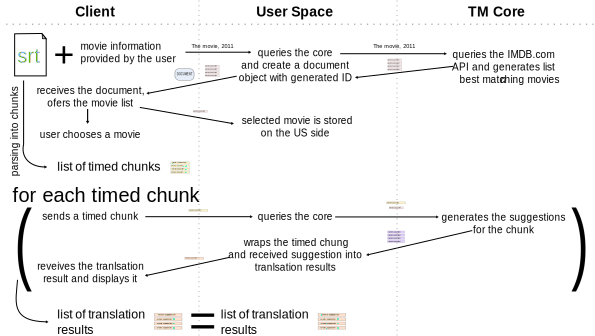
\includegraphics{figures/creating_document.pdf}
\end{center}
\caption{Structure of component communication during a new document creation}
\end{figure}

When a new document is created, the User Space receives a basic information about the movie first. Based on that it creates a Document object and saves it to the database immediately, to receive a unique  database ID which is the used as a document identifier in all other calls. The core is called at this moment to provide a list of possible movies with best matching title and year of production together with genre tags obtained from the Freebase knowledge base. The user is then supposed to choose one or none of the suggested movies. This information is used by the User Space at the moment the core is queried for the translation suggestions.

When a new document is created, the client application starts to send the batches of chunks which are supposed to be translated. When the User Space receives such call, it queries the TM Core for the translation suggestion and adds the chunks to the list list chunks which the appropriate document consists of. Once the suggestion are generated they are thrown away immediately. Keeping a copy of them in memory during runtime and saving them to the database would increase massively the memory requirement and the database size, which can be easily avoided. This also means that when the client queries the saved translation results it will receive them without the translation suggestions. In such case the suggestions are provided by on demand calls per chunk. \todo{refer to the place in GUI documentation}

User Space also provides feedback to the translation memory. A list of new translation the users have produced can be generated together with information which translation pair they used to post-edited is provided to the Data Import module which adds the new translation to the translation memory and use the data also for training the scoring of the suggestions. \todo{Add a reference to the place this is described}

Export of the subtitle files is also solved in the User Space. It is described in more detail in section \ref{sec:export}.

\section{Implementation Details}
\subsection{The Data Types Overview}

The User Space uses the shared data types used thorough the application or the wrapper of such classes. A brief overview of the used classes and their role in the User Space follows. (Prefix US means User Space.)

\begin{itemize}
\item {\tt FilmtitBackendServer}  -- The class is the Java Servlet whose public methods are invoked by the RPC calls. Its main task is to mediate the calls to concrete opened sessions and take care of users login. A thread checking if there some sessions without activity for a long time and termites the non-active sessions is run the server class.

\item {\tt Session} -- The class represents a running session. There is exactly one session object for one logged in user, it is actually the Session class which process the client calls. It contains hash tables of actively edited documents to make them quickly accessible by their IDs. During the existence of a session object all the client side operations are stored just in the memory and saved immediately to the database. When the session ends -- either by the user logging out or by exceeding the maximum time without a user action -- a record about the session is stored to database -- id of the user that owned the session, its start time and end time. This is intended as an activity log from which further statistics can be inferred.

\item {\tt USUser} -- This class is a wrapper of the shared User class. During the existence of the session its used as a provider of the documents owned by the user. It is also used for storing the settings of the user. In advance to the shared class a set of documents which has been left opened when the last user's session was terminated is also stored in the class which is used at the time a new session is created. 

\item {\tt USDocument} -- The class is a wrapper of the shared {\tt Document} class. A {\tt USDocument} object represents a subtitle file with additional information about the movie it belongs to. Its content is supposed to be a mirror image of the Document object on the client side. It contains a list of Translation Results representing the actual subtitle chunks if the document is loaded to be edited. It is not connected to the translation results by the database mapping to make it easy to send the list user's documents without the actual content.

\item {\tt USTranslationResult} -- It is a wrapper for the shared {\tt TranlsationResult} class. The class congregates the original subtitle chunk, its timing, the translation suggested by translation memory and the result of the user activity -- the user's translation which translation suggestion she has chosen. It is the class where the actual translation is being done. Despite a user can delete the document he is working all the translation results are kept in the database to provide a  feed back to the translation memory.

\item {\tt Emailer} -- A class used for sending email from the application. It is used as a confirmation of user registration and also when the user forgets his password and requires sending a new one via email.

\end{itemize}

There are also two third-party classes included in the User Space source code. It is the {\tt IdGenerator} class which generates id sessions (distributed under the {\it Apache License, Version 2.0}) and the {\tt BCrypt} class which ensures hashing the passwords before we store them in the database (distributed under {\it BSD licence}).

The {\tt SubtitleDownloadServlet} class responsible for exporting the subtitle files is described in section \ref{sec:export}. Details concerning the user registration, login and using open ID are discussed in more detail is section \ref{subsec:simple_login} in the GUI chapter. Details about handling the communication with the client are covered in section \ref{sec:communication} of the GUI chapter.

\subsection{Database Mapping}

As was mentioned many times before, the User Space mirrors all the client operations and make them persistent on the server side. The persistence ensured by saving the data to the database. The exist many sophisticated tool for Java to ensure the data persistence, e.g. \emph{Java Persistence API} framework which or some frameworks working on the higher level of abstraction as \emph{Spring Data Framework}. Since only very basic database operations are required during the run of the User Space -- loading and saving of the raw Java object -- only a object relational mapping is library used, namely the \emph{Hibernate}.

The core also uses Hibernate for mapping the {\tt MediaSource} class (gathering information about movie). User Space shares the mapping of such class and uses a class extended from the core class to manage the database transactions.

The mapping just reflects the data properties of classes. If the class is a wrapper of a shared class the getters and setters of the properties are bind to the wrapped objects properties.

As was told before, the mapping of {\tt USDocument} does not include the list of Translation Results the document contains in order to be able to send the documents both with and without the translation results. It would be also possible to use the lazy Hibernate collection mapping, but it would cause problem at the time the object serialized.

\subsection{Providing Feedback to the Translation Memory}

In order to be able provide a feedback to the translation memory and take advantage of the translator work for improving of the translation memory, the implementation of deleting a document a selecting of the media source needs to be done not in a straightforward way. Handling this requirements is described in following paragraphs.

The User Space and the Translation Memory Core use the same database table for the media source (representing the movie or the TV show the subtitles are from). When the user creates a document she is required to enter the title of the movie she is about to translate. After that the {\it Freebase} service is queried for the movies and TV shows possible having such title and a list of this matches is provided to the user to choose from. After the user chooses the media source, the media source object is sent back to the User Space. Then the search in the database table is done. If there is a record with the same title and the release year, its data (genres and thumbnails URL) are updated, if it is a completely new media source, it is saved to the table.

The reason for doing it is not to have duplicate media sources in the database and also the fact that the meta data of the movie should be available to the Data Import module when the feedback to the translation memory is provided.

Another thing to be mentioned here is handling the document deletion. When the user clicks on the delete button in the interface, the document is marked to be deleted in the User Space and is removed from the list of documents owned  by the user and from the list of the documents that has been loaded during a session. From that time the document is not available for the user. After dealing with this a thread is run that deals with the translation results the document consists of. All the translation results that has already provided the feedback to the translation memory are deleted from the database. If the document is empty after this step, it is delete too.

Providing the feedback itself is done by a static method of the {\tt USTranslsationResult} class. This method returns all the translation results what have not been used for feedback before (have {\tt hasSentFeedback} flag set to false. The translation results are provided with a reference they belong to which allows resolve the media source later. If the translation results are form a document that has been flagged as ready to be deleted, both the translation results and the document are delete. Otherwise just the flag informing about having provided the feedback is set.

\section{Exporting Subtitle Files}
\label{sec:export}

TODO \todo{Write it}



\chapter{Communication between GUI and US}
\label{chap:communication}
\label{sec:communication}

This chapter describes the communication interface between the GUI and the Userspace. The central part of the interface are Remote Procedure Calls, described in XXX, YYY and ZZZ, but some of the sequences span more than one RPC: these are further described in XXX.

\section{Remote Procedure Calls}

GUI communicates with Userspace via a GWT RemoteService implementation, defined as the FilmTitService interface.
The interface provides asynchronous RPC methods (the responses are processed by callbacks).

The method is always called from the client, because Javascript security policies do not allow to handle incoming calls.
Therefore, in case the Userspace needs to actively contact the GUI without the GUI having sent a request before,
this has to be implemented in the GUI by polling.

The method always returns an instance of the return type on success or an instance of an exception on failure.
In case of common points of failure that do not qualify as an exceptional state, such as user registration attempt with an already existing username, the common failure is typically signalled by the return value instead (typically a null or a false).

Most of the RPCs can only be invoked by a logged in user. Such RPCs always have the sessionID as their first parameter to authenticate the user and can throw an InvalidSessionIdException.

\section{Manipulating Documents}

TODO: See shared Document, see shared Chunk, see shared TimedChunk.
(Needed to understand e.g. movieTitle or ChunkIndex.)

A document is always identified by its documentID (a long number generated by Userspace on document creation), therefore most of the methods have the documentID as one of their parameters.

A chunk in the document can always be identified by its ChunkIndex, but for convenience in some cases the whole chunk is sent instead.
\todo{we should most probably send only the ChunkIndex always (except for saveSourceChunks of course)}

\subsection{Whole Document Operations}

\subsubsection{DocumentResponse createNewDocument(String sessionID, String documentTitle, String movieTitle, String language, String moviePath)}

Creates the document
(without source chunks, which have to be added by calling saveSourceChunks),
returns its id, together with media source suggestions based on movieTitle.
     	
\subsubsection{Void selectSource(String sessionID, long documentID, MediaSource selectedMediaSource)}
Sets the media source of the document. The media source represents the movie or series which the subtitles come from.

\subsubsection{List<Document> getListOfDocuments(String sessionID)}
Returns all documents owned by the user, ordered by date and time of last change.

\subsubsection{Document loadDocument(String sessionID, long documentID)}
Returns the document with the given id, with source chunks but without translation suggestions (these have to be explicitely requested by getTranslationResults).

\subsubsection{Void changeDocumentTitle(String sessionID, long documentID, String newTitle)}
Sets a different title for the document.

\subsubsection{List<MediaSource> changeMovieTitle(String sessionID, long documentID, String newMovieTitle)}
Returns media source suggestions based on newMovieTitle.
The movie title is not changed yet,
this is only done on calling selectSource.
TODO: is this true?     	 
     	
\subsubsection{Void deleteDocument(String sessionID, long documentID)}
Remove the given document from the list of user's documents.
(The data might not be discarded immediately
as the translations still might be used to enrich the translation memory)	 

\subsection{Source Subtitles Operations}

\subsubsection{Void saveSourceChunks(String sessionID, List<TimedChunk> chunks)}
Save the given source chunks as the contents of the given document
(which was already created by calling createNewDocument).

\subsubsection{Void setChunkStartTime(String sessionID, ChunkIndex chunkIndex, long documentID, String newStartTime)}
Change the start time of the given chunk to the new value. The value must be in the SRT format, i.e. hh:mm:ss,ttt.

\subsubsection{Void setChunkEndTime(String sessionID, ChunkIndex chunkIndex, long documentID, String newEndTime)}
Change the end time of the given chunk to the new value. The value must be in the SRT format, i.e. hh:mm:ss,ttt.

\subsubsection{Void setChunkTimes(String sessionID, ChunkIndex chunkIndex, long documentID, String newStartTime, String newEndTime)}
Change the start time and end time of the given chunk to the values. The values must be in the SRT format, i.e. hh:mm:ss,ttt.

\subsubsection{TranslationResult changeText(String sessionID, TimedChunk chunk, String newDbForm)}
Change the source text of the chunk,
resulting in new translation suggestions
which are sent as the result.

\todo{why dont we send the ChunkIndex and documentID instead?}

\subsubsection{Void deleteChunk(String sessionID, ChunkIndex chunkIndex, long documentID)}
Remove the chunk from the document, together with its translation if it exists.

\subsection{Target Subtitles Operations}

\subsubsection{TranslationResult getTranslationResults(String sessionID, TimedChunk chunk)}
Get the list of possible translations of the given chunk.
The TranslationResult instance contains zero or more translation suggestions, which come from the Translation Memory and/or the Machine Translation System.

\subsubsection{List<TranslationResult> getTranslationResults(String sessionID, List<TimedChunk> chunks)}
Get the list of lists of possible translations of the given chunks.
Each TranslationResult instance contains zero or more translation suggestions, which come from the Translation Memory and/or the Machine Translation System.

\subsubsection{Void stopTranslationResults(String sessionID, List<TimedChunk> chunks)}
Stop generating translation results for the given chunks
(to be called after getTranslationResults has been called
with the given chunks).

\subsubsection{Void setUserTranslation(String sessionID, ChunkIndex chunkIndex, long documentID, String userTranslation, long chosenTranslationPairID)}
Save the user translation of the given chunk (no matter whether it is user\'s own translation or a suggestion taken over or post-edited).
The id of the TranslationPair chosen for post-editing is also sent, providing feedback which then can be used to improve future suggestions.

\section{User Registration and Login}

The user is required to log in to use the application.

The user is logged in if he has a valid sessionID which is linked to a user account.
The sessionID expires after a given period of time without any user interaction with the server,

Two ways to log in are supported -- Simple Login and OpenID Login; these are further decribed separately. The only two common methods are checkSessionID and logout.

\subsubsection{SessionResponse checkSessionID(String sessionID);}
Validates the given sessionID. To be used with a sessionID that does not result from invoking neither simpleLogin nor getSessionID (such as a sessionID stored in a cookie).
Returns a SessionResponse instance containing the sessionID and the User object if the sessionID is valid, or null otherwise.

\subsubsection{Void logout(String sessionID)}
Invalidate the user session with the given sessionID.

\subsection{Simple Login and Registration}
\label{subsec:simple_login}

The Simple Login is the classical implementation of user login. Each user must first register with a unique username and a password of choice. These credentials are then used to log into the application. (The password is to be stored on the server side in the form of a one-way hash.)

The user can also provide an e-mail address for forgotten password retrieval. He then has the option to request a password reset e-mail, based on his username or e-mail address. The password reset e-mail contains a link to a page where the user can set a new password, based on a temporary password change token.

\subsubsection{Boolean registration(String username, String password, String email)}
Register a user with the given username and password, also setting the e-mail address if provided and sending registration info to it.
Returns true on success, false if the username is already taken, and an exception in case of other errors (usually an invalid e-mail address).

\subsubsection{SessionResponse simpleLogin(String username, String password)}
Try to log in the user with the given username and password.
Returns a SessionResponse instance containing the sessionID and the User object on success, or null if the credentials are invalid.

\subsubsection{Boolean sendChangePasswordMail(String username)}
Send a password reset e-mail
to the e-mail address of the user with the given username.
Returns true if the e-mail is successfully sent;
returns false if the username is not registered or there is no e-mail address stored with the corresponding user account.

\subsubsection{Boolean sendChangePasswordMailByMail(String email)}
Send a password reset e-mail to the given e-mail address.
The password reset link is bound to a username;
therefore, if there are multiple user accounts with the given e-mail address,
multiple password reset e-mail are sent to the e-mail address.
Returns true if the e-mail is successfully sent;
returns false if the e-mail address is not registered with any user account.

\subsubsection{Boolean changePassword(String username, String password, String token)}
Set a new password in case of forgotten password.
The temporary password change token must be still valid,
and identical to one sent in the password reset e-mail
to the user with the given username.
Returns true if the password change is successful;
returns false if the token is not valid.

\subsection{Login via OpenID Services}
\label{subsubsec:gui_openid}

The OpenID Login process is described in detail in a separate section \ref{sec:OpenID_Login}.

\subsubsection{LoginSessionResponse getAuthenticationURL(AuthenticationServiceType serviceType)}

Return the URL of a window to show to the user to log in using his OpenID account at an OpenID provider specified by serviceType. It leads to a webpage of the OpenID provider, with the return page set to the FilmTit application, to the AuthenticationValidationWindow page.

A generated temporary one-time identifier, authID, is also included in the response. It is used to pair the authentication process, which takes place in the newly opened window, with the main GUI window.

\subsubsection{Boolean validateAuthentication(int authID, String responseURL);}

Validate the response URL from the OpenID provider, which contains information about the result of the OpenID authentication.

If the authentication is found to have been successful, a new session is generated for the user and paired with the given authID, and true is returned.
Otherwise, the method returns false.

\subsubsection{SessionResponse getSessionID(int authID)}

Check whether the user has already successfully logged in using his OpenID with the given authID.

\begin{itemize}
\item If yes, the corresponding sessionID and User object are returned.
\item If not yet, but the authID is valid, which means that an OpenID login operation is probably still in progress, null is returned.
\item Otherwise, an exception is thrown.
\end{itemize}

\section{User Settings}

There are several settings that the user can change. There is a separate call for each of the settings -- therefore, a set of indivdual calls must be invoked if the user decides to change multiple settings at once, and each of the calls can succeed or fail independently on the results of the other calls.

The settings are stored in the User object and sent to GUI on login, as a part of the SessionResponse which is the result of the methods simpleLogin, getSessionID and checkSessionID. There is no dedicated method to load the settings; checkSessionID is to be used for that purpose.

\subsection{Account and Logging in Settings}

\subsubsection{Void setUsername(String sessionID, String username)}
Change user's username.

\subsubsection{Void setPassword(String sessionID, String password)}
Change user's password.

\subsubsection{Void setEmail(String sessionID, String email)}
Change user's e-mail.

\subsubsection{Void setPermanentlyLoggedIn(String sessionID, boolean permanentlyLoggedIn)}
Stay logged in permanently (for 1 month) instead of 1 hour (sets the session timeout)

\subsection{Translation Workspace Settings}

\subsubsection{Void setMaximumNumberOfSuggestions(String sessionID, int number)}
Set maximum number of suggestions to show for each line.

\subsubsection{Void setUseMoses(String sessionID, boolean useMoses)}
Include Machine Translation results in translation suggestions.

\section{Remote Logging}

The remote logging is used to log messages from GUI on server. The messages are to be printed in the server log and can also be stored in the database.

\subsubsection{Void logGuiMessage(LevelLogEnum level, String context, String message, String sessionID)}
Log the given message from GUI on server.
The suported levels are DebugNotice, Notice, Warning and Error.
The context specifies the type of the message and should be constant for each instance of a similar message; it can contain e.g. a class name, a method name or an RPC name. The message should be as detailed as to provide all necessary information, including e.g. values of variables or a stacktrace if applicable.

The sessionID is only used to include the userID in the logged message; it is to be null if the user is not logged in.

\section{Exceptions Thrown by RPCs}

The RPCs typically throw an exception on failure. These exceptions should be of only four types, described in this section.

\subsection{InvalidSessionIdException}

Most of the RPCs can only be invoked by a logged in user -- such RPCs take the sessionID as their first parameter and throw an InvalidSessionIdException in case of an invalid sessionID. Typically the ID would be originally valid but expired, so the expected reaction to this exception is to simply ask the user to log in again.

\subsection{InvalidDocumentIdException}

RPCs that manipulate the document usually take the documentID as a parameter and throw an InvalidDocumentIdException if a document with the given ID does not exist or does not belong to the user.

\subsection{InvalidChunkIdException}

RPCs that manipulate individual chunks take either the whole chunks or only their indexes as a parameter. They throw an InvalidChunkIdException if the specified chunk does not exist.

\subsection{InvalidValueException}

The InvalidValueException is thrown by a method if a value provided by the user, such as an e-mail address or a password, does not have the required format. It always contains details about the nature of the error as the message, which usually should be shown to the user.

\section{Complex Operations}

In most cases, one RPC is sufficient to perform the whole operation. However, sometimes a whole sequence of several RPCs is required to complete one complex operation. Such operations are described in this section.

\subsection{Document Creation}

see \ref{rpc:sd:document_creation}

\todo{describe textually}

\todo{probably translation suggestions generation does not belong here}

\begin{figure}[h]
\begin{center}
\includegraphics[scale=0.65]{figures/document_creation_sequence_RPC.pdf}
\end{center}
\caption{Sequence diagram of document creation, including translation suggestions loading.}\label{rpc:sd:document_creation}
\end{figure}

\subsection{OpenID Login}
\label{sec:OpenID_Login}

This section describes the OpenID Login process, which is also shown in the sequence diagram \ref{rpc:sd:openid_login}.

The authentication itself is done in a new authentication window.
A successful authentication in the authentication window is then paired with the GUI main window using a temporary one-time identifier, authID, shared by the Userspace, the main GUI window and the authentication window.
(Because of Javascript security restrictions, there is no simple way of sending the result of the authentication process from the authentication window to the main window;
however, the authID can be sent to the new window easily because it is already known at the time of its creation.)

When OpenID Login is requested by the user, the GUI main window calls getAuthenticationURL.
The Userspace generates an authID, and a URL to be used for the authentication, and returns that to the GUI, which opens a new authentication window with the received URL.
The URL points to an OpenID provider webpage (currently supported OpenID providers are Google, Yahoo and Seznam). As a GET parameter, it contains the return URL, which leads back to FilmTit -- to the AuthenticationValidationWindow page, including the authID as a GET parameter in the return URL.

After opening the authentication window, GUI starts waiting for the user to authenticate. The waiting is active, polling the Userspace with getSessionID in regular intervals until a non-null value is returned.

Meanwhile, the user can authenticate in the authentication window. The OpenID provider then redirects the user to the return URL, which is the AuthenticationValidationWindow, together with parameters describing the result of the authentication and providing some information about the user (see \todo{link to userspace} for details).
The whole response URL is then sent through validateAuthentication to Userspace for validation.

If Userspace finds the authentication to be successful, a new session is created for the user, and the sessionID is stored in a pair with the authID.
If a user with the given OpenID is not registered yet, registration is transparently performed at this moment (see \todo{link to userspace} for details); no explicit registration is required for OpenID login.
The authentication window is then closed.
In case of an error, the error message is displayed in the authentication window (and the window stays open).

When a successful authentication took place, the getSessionID method returns the sessionID and a User object, the polling stops and the authentication process is completed.

\begin{figure}[h]
\begin{center}
\includegraphics[scale=0.55, angle=90]{figures/openid_login_sequence.pdf}
\end{center}
\caption{Sequence diagram of OpenID login.}\label{rpc:sd:openid_login}
\end{figure}


\chapter{Graphical User Interface}
%% ----------------------------------------------- %%
%%            Graphical user interface             %%
%% (documentation chapter for the FilmTit project) %%
%% ----------------------------------------------- %%

The Graphical User Interface (GUI) is the part of the application that is loaded by the user in his web browser. It is written mostly in Java but compiled by the Google Web Toolkit (GWT) into JavaScript. Its main tasks are

\begin{itemize}
\item visualisation of the application and communication with the user in a user-friendly way, especially providing an efficient translation workspace adapted for translation of movie subtitles
\item communication with the User Space (see Chapter~\ref{chap:userspace}) through the Remote Procedure Calls (see Chapter~\ref{chap:communication}), especially to provide the user with translation suggestions from the core translation memory (see Chapter~\ref{chap:core}) and for data persistence
\end{itemize}

\section{Goals}
% (Honza)
Our main goal is to offer a tool for the translators of the movie subtitles as easy and effective to use as possible. With the capabilities of the current web browsers, we decided to make FilmTit a web-based application, therefore sparing the user the need to download and install anything.

\section{Google Web Toolkit}
% (Honza and Ruda)
The web-based user interface representing the client part of the FilmTit application is based on the Google Web Toolkit (GWT) framework. This technology is a development toolkit for building and optimizing browser-based applications %\citep{Gwtweb}
and is based on the idea of compilation of Java source code into JavaScript. Therefore, it enables us to write in Java even on the client side, but preserving most of the advantages of web application accessibility for the user.

The official description of GWT is as follows:

Google Web Toolkit (GWT) is a development toolkit for building and optimizing complex browser-based applications. Its goal is to enable productive development of high-performance web applications without the developer having to be an expert in browser quirks, XMLHttpRequest, and JavaScript. GWT is used by many products at Google, including Google Wave and the new version of AdWords. It's open source, completely free, and used by thousands of developers around the world.

More about decision for using GWT can be found in \ref{subsubsec:implementation:gwt}.

\subsection{Browser Support and Optimization}
GWT also provides a feature which makes the final web application similar in different major browsers and optimized to a certain degree for each of them. This feature is called {\em deferred binding} and it is based on generating different versions of the JavaScript code during compile time, only one of which needs to be loaded by a particular client browser at runtime. This process is by default maintained by the GWT compiler itself, so that the developer does not have to worry about it.

However, this ``unification'' is not complete, nor it is intended to be. It covers only the bigger and more crucial differences of the code behavior among various browsers, but does not address some slight variancies e.g.\ in design of the basic elements (and their most common behavior). This seems reasonable, because forcing each browser to interpret the code in the exact same way would mean hardcoding almost everything from scratch and not using many of their provided features, which would be probably impossible anyway. Nevertheless, some of these ``slight differences'' which we have encountered proved to be quite crucial for our intended design (especially in the event-handling domain), so lots of work had to be done to reasonably unify the application's behavior even among the major browsers.

Still, our hope is that GWT development will continue and will keep up with the development of web browsers, allowing us to provide browser-up-to-date versions of FilmTit simply by acquiring a new version of GWT and recompiling the project. Currently, the application works well with Opera v.~12
Firefox v.~14, Chrome v.~21 and Safari v.~5.1.5 or higher.


\subsection{Designing by UiBinder}
Another very useful and comfortable feature of the GWT for designing the user interface is the UiBinder. The idea behind this approach is to design the visual structure of the page (or its part) in an HTML-like way (this is called the {\em UiBinder template}) and its behavior and functionality in a Java class (called the {\em owner class} for the template). The UiBinder itself is then an object binding these two approaches together. This style of creating the web application supports the respected best practice to divide the visual design and the functionality. It also allows to create the web page's appearance in a way which is more natural to web designers (e.g. HTML-like), as well as more readable and modifiable. Other advantages include supposedly better performance (as the browsers can better optimize the rendering from the UiBinder templates than from the heavier-weight Java-based widgets and panels) and support for internationalization (not used by FilmTit at the moment).

The actual source code of a page designed this way (or of its segment) then consists of a file with the *.ui.xml Ui-Binder template (where also the style definition can be included directly) and a corresponding *.java owner class, where the elements of the template can be accessed as widgets (as well as made accessible to other classes). The owner class then can be simply instantiated and plugged into an existing design just like any other widget.

\subsection{Twitter Bootstrap Library}
For enhancing the visual appearance of our application to a modern look without a professional graphic designer, we have decided to use an existing open-source library for GWT which displays the page elements (and their groups) in the style of the Twitter pages. This library is called GWT-Bootstrap and is easily applicable with the UiBinder-style designing. It is also still a live project, so there is a hope that more features would be available in the possible future development.

Similarly to other third-party libraries used by FilmTit, the GWT-Bootstrap library is attached as a Maven dependency and downloaded automatically from its own Maven repository.


\section{GUI Structure}
% (Honza/Ruda)

The GUI is contained in the package {\tt cz.filmtit.client} (not {\tt cz.filmtit.gui} for ``historical'' reasons -- ``client'' is the default package name in GWT for the client side of a web application). All of it is written in Java (in its subset that is GWT-compilable to JavaScript), with occasional methods with bodies written directly in JavaScript (for reasons clarified in \ref{subsubsec:implementation:gwt}). Thus, the GUI can actually only be compiled to Javascript.

The GUI also makes use of the shared classes (package {\tt cz.filmtit.share}, see~\ref{sec:shared_classes}), which are written using only the intersection between standard Java and GWT-compilable Java and are therefore fully compilable both to Javascript and to Java bytecode.

Some settings have to be done via several resource files in the webapp directory. (This is required by the Java Servlets technology used to deploy the application.)

\subsection{Gui.java}

The main class is Gui.java. It defines the web application itself, providing an entry point, initialization methods, logging methods and access to page switching. It also contains fields that are considered global, such as the {\tt sessionID} of the currently logged in user.
It behaves as a static class, except for the {\tt onModuleLoad()} method required by GWT, which corresponds to the {\tt main()} function.

\subsection{Pages}

The subpackage {\tt cz.filmtit.client.pages} defines the pages of the application.
Please refer to the sitemap figure \ref{fig:sitemap} for an overview of the pages, which are:

\begin{itemize}
\item {\tt DocumentCreator}, used to create a new document
\item {\tt TranslationWorkspace}, the main page of the application where the actual translations take place
\item {\tt UserPage}, providing listing of user documents and the possibility to edit them
\item Settings, enabling the user to change several settings, such as his password or the maximum number of translation suggestions to show
\item {\tt WelcomeScreen}, displayed as the first page of the application
\item {\tt About}, showing basic information about the applicaton
\item {\tt PlayerInfo}, showing guidelines on how to run the media player
\item {\tt ChangePassword}, used as the target of the password change link sent by e-mail to users who forget their password, enabling them to set a new password
\item {\tt AuthenticationValidationWindow}, a special page that receives OpenID authentication data from an OpenID provider and passes them to User Space for validation
\item {\tt Blank}, a special page with no contents and is used to temporarily hide the contents of another page
\end{itemize}

\begin{figure}
\begin{center}
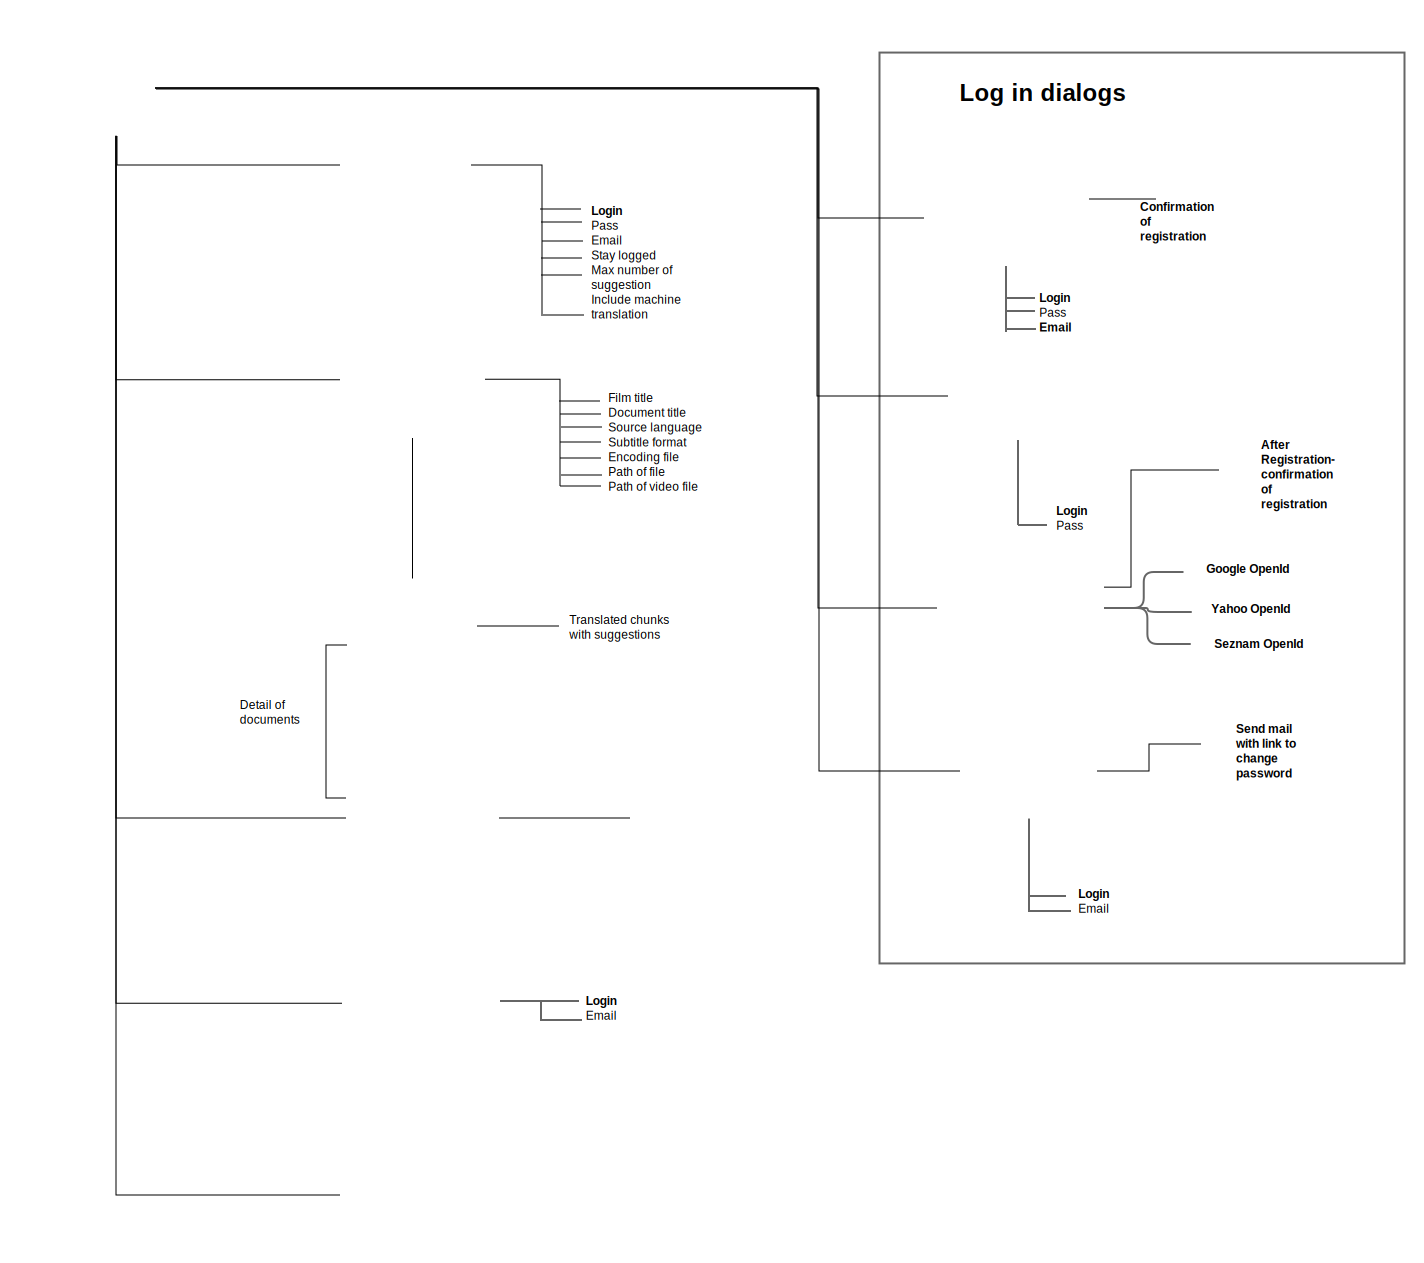
\includegraphics[scale=0.4]{figures/sitemap.pdf}
\end{center}
\caption{Site map of the application}
\label{fig:sitemap}
\end{figure}

As was already mentioned, each page has its layout and function separated as much as possible, with the function being defined in a <page>.java file and the layout in a UiBinder <page>.ui.xml file.

The pages package also contains the {\tt GuiStructure}, which defines the content panel, into which the individual pages are loaded, and the top menu, which enables the users to log in and out and to switch pages.

A page is created and loaded by calling its constructor, which may require some parameters (such as {\tt documentID} for {\tt TranslationWorkspace}).
Page loading and switching is handled by the {\tt PageHandler}, which also provides support for URLs: e.g.\ the About page can be accessed by a URL {\tt http://server/\#About} or {\tt http://server/?page=About} (the first one being the default), with the help of the GWT History class.

\subsection{Dialogs}

Apart from pages, the GUI also contains several dialogs that can be displayed on top of a page. The dialogs are defined in the {\tt cz.filmtit.client.dialogs} subpackage and are typically extended from the abstract {\tt Dialog} class in the same package.

The {\tt Dialog} class defines a modal dialog container and an ``interface'' to be used to handle the dialogs -- all dialogs should only be accessed via this interface (except for their creation, which is invoked by their constructor).
The interface methods are especially
{\tt deactivate()}, {\tt reactivate()}, {\tt showInfoMessage()}, {\tt showErrorMessage()} and {\tt close()}. To deactivate a dialog means to disable all of its active elements so that the user cannot interact with it and must wait for the dialog being reactivated or closed.

The Dialogs defined by the application are:
\begin{itemize}
\item {\tt LoginDialog}, used for logging in and related functions,
\item {\tt SessionIDPollingDialog}, used when waiting for OpenID login process to complete,
\item {\tt MediaSelector}, used to select the correct movie or series of a newly created document,
\item {\tt TimeEditDialog}, used to edit timing of subtitle items,
\item {\tt DownloadDialog}, which enables the user to download the translated subtitle file,
\item {\tt GoingOfflineDialog}, offering the user to turn on the Offline Mode, and
\item {\tt GoingOnlineDialog}, offering the user to upload data from Offline Mode when the user goes back online
\end{itemize}

\subsection{Remote Procedure Calls Implementation}

Each RPC is in GUI represented by a class from the {\tt cz.filmtit.client.callables} subpackage. The name of the class is typically similar to the RPC name -- e.g.\ for {\tt deleteDocument} RPC it is the {\tt DeleteDocument }class. Each of these classes is extended from the {\tt Callable superclass}, which will be described in the next section.

The RPC is invoked by creating a new instance of the callable class, providing the neccessary parameters in the constructor -- e.g. to invoke the {\tt simpleLogin()} RPC with the username and password parameters, one simply calls {\tt new SimpleLogin(username, password)}. A reference to the instance usually does not have to be kept, since the actions to take on success or failure of the RPC are already hard-coded into the onSuccessAfterLog and onFailureAfterLog methods of the class.

\subsubsection{Callable}

The institute of the {\tt Callable} superclass of all RPC classes has several purposes:

\begin{itemize}
\item to alleviate the burden of boiler-plate RPC invocation code by providing a wrapper for the ``raw'' RPC call
\item to provide utility methods and default actions, such as error handling
\item to provide actions to be always taken, such as logging of the calls with their parameters, and their results
\item to provide a common structure for all RPCs
\end{itemize}

The Callable class itself implements the {\tt AsyncCallback} interface, implementing the required {\tt onSuccess} and {\tt onFailure} methods; therefore, and instance of its subclass can be directly passed to the asynchronous call as the callback.

The subclasses representing the individual calls must only override the {\tt call()} method, which specifies the actual RPC to be invoked.
They can also modify the default behavior defined by the superclass by overriding several other methods, such as {\tt onSuccessAfterLog}, {\tt onEachReturn}, {\tt onFailureAfterLog}, {\tt onProbablyOffline} etc. This way, the behavior needed can be always achieved, but the default implementation is often sufficient, so the subclasses often override only one or two methods, keeping their code as simple as possible. (The method most often overridden is the {\tt onSuccessAfterLog} method; its default implementation is to do nothing, which is only good for RPCs that do not require any reaction of GUI on their successful return, such as {\tt changeDocumentTitle} or {\tt stopTranslationResults}.)

\subsubsection{Error Handling}

If the request fails for any reason, it is retried by default; four attempts are made for each request, always retrying after a short time interval.
Resending the request is the default behavior which the subclasses override in cases where it is obvious that resending will not help (e.g. incorrect e-mail address format or an already existing username on registration).

In case of network problems, both temporary and permanent (this cannot be easily distinguished), the GUI usually receives a {\tt StatusCodeException} with the status code 0. In such case the request is always resent three times before passing control to the {\tt onProbablyOffline} method (this behavior cannot be overridden).

There is also a timeout for each request after which the request is regarded as lost and is retried.

The default action in case of an error is to show the error message in a JavaScript alert window, except for the {\tt InvalidSessionIdException} where the default action is to ask the user to log in again.
The subclasses often override this by showing the message in a Dialog (invoking the {\tt reactivateWithErrorMessage} method of the {\tt Dialog} class), or by ignoring the error completely (e.g.\ when deleting a document, a failure with an {\tt InvalidDocumentIdException}, meaning that the document does not exist, is an error, but there is no need to inform the user because the result is the same as if the RPC succeeded: the document does not exist now.)

Most of the RPCs contain the {\tt sessionID} as one of their parameters to authenticate the user. All of such RPCs can thus throw an {\tt InvalidSessionIdException}, to which the default action is to show the Login Dialog to the user.

\subsection{Offline Mode}

The Offline Mode offers the users the possibility to continue translating a document even without a connection to the server. Their translations are stored locally in his browser and sent to User Space once they go back online.
Support for storing the data is ensured by the HTML5 Local Storage feature, which provides an in-browser data storage, accessible from JavaScript.
Each object is stored as a pair of a unique string key and a string value (therefore, serialization to string is necessary to store complex objects).

The Offline Mode support is separated into three parts: the {\tt LocalStorageHandler}, the {\tt Storable} interface, and classes implementing the interface (i.e. the {\tt SetUserTranslation} class).

\subsubsection{Storable interface}
\label{gui:subsubsec:storable}

This interface defines methods that need to be implemented by a class to be storable in the Local Storage, especially:

\begin{itemize}
\item {\tt toKeyValuePair()} -- to serialize the object into a pair of a key and a value

\item {\tt static fromKeyValuePair(KeyValuePair)} -- a factory method that deserializes the object from a pair of a key and a value (not actually defined by the interface; for a discussion on that matter see Section~\ref{ip:subsubsec:offline})

\item {\tt onLoadFromLocalStorage()} -- invoked by the {\tt LocalStorageHandler} when the user decides to upload the object
\end{itemize}

Each implementing class defines its serialization such that its key uniquely identifies the object and the value contains all data (except for those already contained in the key) needed to reconstruct the object.
(The key and the value are expected to consist of semicolon separated fields by default, but each class can define its own serialization, there are no restrictions other than defined by the String class.)

To store in the Local Storage, the key is extended to a ``full key'' by adding the {\tt classID} (e.g.\ ``SetUserTranslation'') and the {\tt userID} (a long),
so the resulting format of key is:

\begin{center}
full key = {\tt userID@classID:key}
\end{center}
When loading the object from the Local Storage, these added fields are used to indetify the owner of the object and the class to deserialize the object into, and are stripped before passing the key to the {\tt fromKeyValuePair()} method; thus, the class gets the key for deserialization in exactly the same format as it was produced by the class on serialization.

Unlike the key, the value is defined solely by the implementing class and is stored and loaded ``as is''.

The {\tt Storable} interface is currently only implemented by the {\tt SetUserTranslation} class, for reasons described in the Implementation Process chapter, section~\ref{par:process_serialization}.

\subsubsection{SetUserTranslation}

The {\tt SetUserTranslation} class defines its serialization key and value as follows:

\begin{itemize}
\item key = {\tt documentId;chunkId;partNumber}
\item value = {\tt chosenTranslationPair;userTranslation}
\end{itemize}

The onLoadFromLocalStorage() method implementation invokes the setUserTranslation RPC.

\subsubsection{LocalStorageHandler}

The static {\tt LocalStorageHandler} handles storing and loading of Storable objects to and from the Local Storage.

An important field is a boolean ``online'', which determines whether user is in Online Mode or Offline Mode. Setting this value is eqivalent to switching the Offline Mode on or off.

The {\tt LocalStorageHandler} implements especially the following (static) methods:

\begin{itemize}
\item {\tt storeInLocalStorage} (Storable) -- takes a Storable object, serializes it and stores it into the Local Storage

\item {\tt loadUserObjectsFromLocalStorage()} -- examines the Local Storage and returns a list of objects that belong to the current user

\item {\tt uploadUserObjects()} -- deserializes the loaded objects and invokes their onLoadFromLocalStorage() methods
\end{itemize}

\subsubsection{The Offline Mode operation}

Please see the sequence diagram \ref{gui:sd:offline_mode_1} for the first phase, where the user goes offline and continues working on the translation, and the sequence diagram \ref{gui:sd:offline_mode_2} for the second phase, where the user goes online again and the locally stored data are uploaded to the server.
(For simplicity the diagrams do not show some implementation details;
also, parameters are listed only if they are necessary for understanding the process.)

\begin{figure}[h]
\begin{center}
\includegraphics[scale=0.55]{figures/offline_mode_1.pdf}
\end{center}
\caption{Sequence diagram of turning on the Offline Mode and translating the document in Offline Mode.}\label{gui:sd:offline_mode_1}
\end{figure}

\begin{figure}[h]
\begin{center}
\includegraphics[scale=0.55]{figures/offline_mode_2.pdf}
\end{center}
\caption{Sequence diagram of the user going online after using Offline Mode.}\label{gui:sd:offline_mode_2}
\end{figure}

Before using the Local Storage, it is checked whether it is supported -- if it is not, Offline Mode is not offered to the user and a relevant message is displayed.

When a setUserTranslation call fails with the ``probably offline'' error, it is saved into a queue of failed calls that are to be stored offline if the user agrees (other {\tt setUserTranslation} calls could already have been invoked and will also fail and get enqueued). If the user decides to turn on the Offline Mode, all calls from the queue are stored into Local Storage.

In Offline Mode, the style of the menu is changed and all active components are hidden, because the user should not leave the Translation Workspace while in Offline Mode. Also, going back or forward using the browser controls is disabled: each upcoming page switch is cancelled.

The {\tt SetUserTranslation} calls invoked while in Offline Mode are not sent to server, but they are serialized into a key-value pair and stored in the Local Storage.

Once the user is back online and logs in again, the {\tt LocalStorageHandler} examines the Local Storage. It strips the {\tt userID} part of the key of each object found and compares it to the currently logged in user. If some data belonging to the users are found, they are informed about their count and are suggested to upload the data. If they agree, {\tt LocalStorageHandler} goes through the data, stripping off the ClassID and invoking the corresponding ``{\tt ClassID.fromKeyValuePair()}'' deserialization. Subsequently, the {\tt onLoadFromLocalStorage()} method is invoked on each of the resulting objects -- the {\tt SetUserTranslation} implementation of this method is to invoke the {\tt setUserTranslation call}, i.e.\ to store the translation on the server. When the call returns, {\tt LocalStorageHandler.SuccessOnLoadFromLocalStorage()} or {\tt LocalStorageHandler.FailureOnLoadFromLocalStorage()} is called, as required.

When each of the loaded objects has either succeeded or failed, the user is informed about the result. In case of errors, he can decide to retry loading the failed data or to delete them.

\subsection{SubgestBox}

An important class is the {\tt SubgestBox}, or ``SUBtitle sugGESTion BOX'', which visualizes the TM results, offering a variety of means of navigation through them.

\subsection{Playing the movie files}

From the beginning, we wanted to be able to show the user the movie file along with the translations. However, legal issues, bandwith issues and disk issues bar us from actually uploading the files to our servers -- so, we tried to implement some kind of playing the users' movie files, from their disks, in the browser, and then communicating with this player via JavaScript, so we can somehow connect it with the translation GUI.

For this, we have to deal with two problems.

\subsubsection*{Video Playback (VLCWidget)}
Playing the movie locally, from disk, is actually the lesser problem. We use VLC browser plugin for that.

VLC\footnote{\url{http://www.videolan.org/vlc/}, short for VideoLan Client} is a popular open source media player. One of its advantages is that it can handle almost any video format and any codec available.

VLC has also feature called ``browser plug-in''\footnote{For some reason, its name is different across VLC documentation. Sometimes, they use the name ``Mozilla plug-in'', sometimes ``Web plug-in'', sometimes ``browser plug-in''.}. The browser plug-in is not a part of standard VLC installation, but can be installed easily.

This browser plug-in can be used for playing local files, in the browser, given that the file address is known. It is possible to rewind forward/backward/stop, all through JavaScript.

There are some slight difficulties in the plug-in, though. One of them is, that it is not possible to jump on an exact time location in the video file. Most video files have so-called seek frames, which can appear more or less often (depending on the setting of the encoder), and VLC plugin always moves to the closest preceding seek frame. The difference can be quite big (even up to 20 seconds). This bars us for playing exactly the time slot of a given subtitle.

The other difficulty is that sometimes, the plugins just freezes without any warning after a move to a position. We have found out that it is somehow connected to the files played; with the exact same movie files, the exact same positions cause the player to crash, but slightly moved positions are all right.

The first issue is solved by not playing just the part with one subtitle, but bigger, 30 seconds ``windows''. The entire movie is split to these 30 second windows, and once the user switches in the {\tt TranslationWorkspace} from subtitle in one window to a subtitle in another window, the whole new window is played. It is actually better than playing just the time of the subtitle, since the user has more context to translate the movie's sentences.

The second issue is solved by detecting the crashes and restarting the whole plugin in the case of crash with slightly moved windows.

All is implemented in \texttt{cz.filmtit.client.widgets.VLCWidget}. Apart from that, the \texttt{VLCWidget} displays the subtitles on the left and on the right of the VLC browser plugin (original on the left, translated on the right).

We intentionally did not implement very sophisticated controls for the player (since it would make the design too complicated). All the player can do is replay the whole current window or pause the playing.

\subsubsection*{Java applet for reading the filename}
The bigger problem is actually \emph{reading the name of the file} before giving it to VLC player plugin.

The browsers are generally built to give pages as little access to user's system as possible (understandably so). That includes the file paths of the files. Even the recent HTML5 standards, that do have access to the file itself, cannot read the filename.

The only way we found, that would be usable across the browsers and systems, was to use a Java applet. Java applets have access to users' disk and can read the filenames; they have to be signed by a certificate, but that certificate can be self-signed.

This is implemented in \texttt{cz.filmtit.client.widgets.FileLoadWidget}.

The problem with this approach becomes evident -- we are now dependent on two external, non-standard, separate plug-ins for the task of playing video files -- VLC plugin and Java plugin. Both have to be installed separately, both often cause issues in various browsers (not only in theory). On the other hand, we achieved the almost impossible task -- playing movie files from users' disk on their browsers. When the is warn users that this functionality is experimental and carefully explain them the two plugins and their installation, we believe the current implementation is acceptable.


\subsection{Parsing and segmentation}
We already wrote about parsing in the chapter~\ref{parsing_subs}. As we mentioned there, we are reusing the same classes for {\tt dataimport} module (where we parsed and segmented thousands of files) in the GUI.

More information about the parsing can be found in the chapter~\ref{parsing_subs}.

\section{Typical Usage}
% (Honza)

\todo{update, some things changed...}

\subsection{Document Creation}

In the most typical case, users (already registered) will open the page with FilmTit and log in. Then, they will go to the {\tt DocumentCreator} page to create a new document. A document corresponds to one movie, or more precisely, to one subtitle file being translated from one language to another. On this page, the users should specify the title of the movie (or series), the direction of the translation (e.g.\ from English to Czech) and provide the actual local file with the source subtitles. They can also set a document title different from the movie title, and set a file path to the corresponding movie video file on his file system.
These information are sent to the User Space and, after refining the movie specification through the {\tt MediaSelector}, the new document is created and the page switches to {\tt TranslationWorkspace}, filled with source subtitles (segmented to chunks) together with their timing on the left side and corresponding empty translation text-boxes on the right side.

See also the corresponding sequence diagram \ref{gui:sd:document_creation}.

\begin{figure}[h]
\begin{center}
\includegraphics[scale=0.40]{figures/document_creation_sequence_GUI.pdf}
\end{center}
\caption{Sequence diagram of document creation.}\label{gui:sd:document_creation}
\end{figure}

\subsection{Document Translation}
\label{sec:document_translation}

At the same time, the subtitle chunks are sent through the User Space to the Core, where the appropriate translation suggestions are generated for them and sent back. When received in the GUI, each translation result is set to the {\tt SubgestBox} corresponding to its chunk, and can be displayed on activation of the translation text-box as a pop-up, with the suggestions sorted according to their estimated accuracy.
The user can then choose any one of them (or none) and edit it (if necessary) to get the translation of the particular chunk. When the users leave the translation text-box, their translation is sent to the User Space through the {\tt setUserTranslation} call to be saved as the user translation of the chunk.

See also the corresponding sequence diagram \ref{gui:sd:document_translation}.
(Some technical details are ommitted for simplicity.)

\begin{figure}[h]
\begin{center}
\includegraphics[scale=0.45]{figures/document_translation_sequence.pdf}
\end{center}
\caption{Sequence diagram of document translation.}\label{gui:sd:document_translation}
\end{figure}

\label{part:manuals}

\part{Development Process Documentation}

\chapter{Implementation and Development Process}
\section{Timeline}

The following section describes the project development, progress and decisions we took through the time the project was developed. After a series of informal meetings, the project officially started in February 2012 and was submitted in September 2012.

\subsection{Initial Project Meetings and Early Implementation Decisions}

The regular project meetings where we discussed mostly the organizational aspects and the top-level design of the application started in December 2011. We easily agreed that we were aiming to create an application quite similar to Google Documents. We have decided very early to use a multi-tier architecture consisting of

\begin{itemize}
\item core translation memory,
\item user space,
\item graphical user interface,
\end{itemize}

\noindent which became very soon separate Maven modules, as we soon started using Maven for building the project.

After overcoming the problems connected with learning the new technology, we became quite satisfied with the decision to use Maven, because it enables to easily combine the parts of the project.

\subsubsection{Project structure}

Despite the fact that we added further modules later, we consistently kept the initial project separation into \emph{Core}, \emph{User Space} and \emph{GUI}. At the beginning, we also assigned team members to different parts of project, which remained relatively stable as well.

\subsubsection{Initial data}

Before receiving the data from OpenSubtitles.org, we were thinking about the source of data to fill the translation memory for the first time. There were several options -- either using the subtitle part of the Czech-English parallel corpus CzEng developed at ÚFAL \footnote{\url{http://ufal.mff.cuni.cz/czeng/}}, using sentences from a general purpose parallel corpus or getting the data from a subtitles server.

\subsubsection{Programming languages}

From the very beginning, we intended to base the project on Java, mainly because there are a number of web technology projects based on Java and
 every team member was familiar with the language. 
We also decided to combine the code in Java and Scala programming 
languages. At that time, there was 
only one team member who knew the Scala language. Although we 
repetitively expressed believes that everyone of us would learn it, at 
the end there was only one other person familiar with the Scala language.

The decision to use both Java and Scala appeared to bring a number of 
complications. On one hand, Scala allows to write concise and efficient 
code; on the other hand, most project members were not able to learn 
Scala sufficiently even to understand the Scala code properly, let alone 
actively producing Scala code, and only used Java.
Although the interoperability between Scala and Java works well in most 
cases because both are based on the JVM, some problems remain. One of the 
problems of interoperability was, for example, that a \emph{List} object 
created in Scala is not compatible with Google Web Toolkit, which expects 
a standard Java \emph{List} implementation.

\subsubsection{Technology for the Client: Google Web Toolkit}
\label{subsubsec:implementation:gwt}

Much more complicated to agree on was the technology of the client. There were many different opinions, from writing the client in {\it PHP} with {\it Nette Framework}, which some of us knew well, to using the {\it JSP} to have all the code consistently in Java, even to quite an extreme idea to make the whole application a {\it Java Applet} (this idea had appeared because of the intention to integrate the video player in the application, since at that time we did not know any other way to do that except creating a Java applet). Finally, we decided to use {\it Google Web Toolkit}, which no team member had any prior knowledge of, but it promised making the communication between server and client and many other things very easy. 

More information about the decision for using GWT and a discussion of its advantages and disadvantages can be found in Section~\ref{sec:reasonsForGWT}.

%Similarly to the Scala language problem, we ended up with only three people able to work efficiently with the Google Web Toolkit. Fortunately, this did not became a bottleneck of the development process.

% I guess me (Ruda) and Honza have probably mastered GWT, but Karel is also quite fluent in it



\subsection{Early Development Process}

Luckily for us, we very soon received a database from {\it opensubtitles.org} containing all the Czech and English subtitle files that were at the server at that time. Soon after that we started working on an alignment algorithm to retrieve the parallel data from the subtitle files (the process is described in Section~\ref{sec:aligning_subtitles}) and enable us to start experiments that helped us to decide which database system could be used.


\subsubsection{Database system}

Choosing an appropriate database system was also an intensively discussed issue. The database underlying the Translation Memory plays a crucial role for the whole system performance. Also using built-in features could save us a lot of additional work.
We evaluated different DBMS and decided to use \postgres~(see Section~\ref{sec:dbms} for details). To test its applicability for our project, we ran several small evaluations of \postgres~features that might be useful to us, e.g.\ the full-text search. As soon as we made the final decision on which DBMS to use, we refactored the evaluation code into {\tt TranslationPairSearcher} classes and started to set out the general architecture of the core. The {\tt BackoffTranslationMemory} class was added and the candidate search was finished in its early stages, so a basic version of the system could be used even though there were no sophisticated rankers yet. For more details on the core architecture, please see Section~\ref{sec:corearchitecture}.

Not having any experience with the object-relation mapping libraries in Java, we decided to use {\it Hibernate}, based on advice from both Internet forums and some of our colleagues.


\subsubsection{Data alignment}

Originally, all the algorithms processing the data we retrieved were implemented in Perl, and the code for importing the data was in the \emph{Core} module, implemented in Scala. Later, to make the code more consistent, we decided to move the data preparation and data import to a separate \emph{dataimport} module and to re-implement the Perl scripts in Scala.

\begin{figure}[h]
\begin{center}
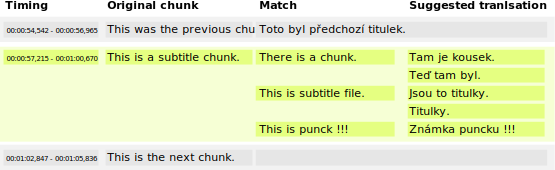
\includegraphics{./figures/original_strucutre.pdf}
\end{center}

\caption{Scheme of the originally intended structure of work with the translation memory. It reflects the original User Space structure and also schematically the original client design.}\label{fig:original_scheme}

\end{figure}

\subsubsection{Video playback}

Very soon, we started to try to solve the video playback in the browser, which we expected to be a really challenging issue. We did some research about \emph{Adobe Flash} technology. We were also thinking about creating a hybrid solution -- an application wrapper with a web browser inside, capable to ensure the video playback for the inner web application.

We very soon had toy implementations of:

\begin{itemize}
\item a player using VLC plugin, to be incorporated into the web application
\item a player as a desktop application, showing the web application in a frame (see Figure~\ref{fig:figures_desktop-app-player})
\end{itemize}

\begin{figure}[h!]
	\centering
		\includegraphics[width=7cm]{figures/desktop-app-player.png}
	\caption{Screenshot of Qt-based desktop application.}
	\label{fig:figures_desktop-app-player}
\end{figure}

We decided for the web application-only version, with no desktop variant, because, observing the development trends, it seems to us that the present and future of applications is in web applications. The benefits are e.g.\ that the learning curve is typically better for a web application, where the user is already familiar with most of the controls and work patterns, installation is not required, so anyone can start using the application immediately, it is easy to use OpenID registration.

Still, there are disadvantages, especially the cross browser support issues, limited power, and larger bandwidth consumption.
An added advantage of GWT is that the bandwidth consumption is actually closer to that of a standalone desktop app, because the application itself is stored in one JavaScript file, which is downloaded at the beginning (similar to installing a desktop application, but it is done transparently), and the rest of the client-server interaction is done through RPCs (basically the same way as it would be done in a desktop application).

An issue we encountered in developing the player and were not able to combat completely is letting the user choose a media file and passing its full file system path to the player. We found out that although it is quite easy to load a whole file from disc into memory, only its filename is passed to JavaScript instead of the full path for security reasons. We did a thorough search on the Internet but found out that there is most probably no clean way around this restriction.

Ultimately we came up with 3 solutions, but none of them pleased us enough:

\begin{itemize}
\item the user inputs the full path as a string into an input box; works well but is not user-friendly (most users probably do not even know that such a thing as a file path exists)

\item the user chooses the file in the file browser and then copies the file path from the browser input box into a textbox; this is probably even less user-friendly

\item a Java applet is loaded to choose the file as Java applets do not have such restrictions as JavaScript, and then passes the path to the application; it seems to us too heavy-weight to create and load a whole applet only to get the file path, but it works quite well -- except for the users who do not have Java installed and working properly (we have also encountered an alternative using Flash for the same purpose, but we still prefer using Java to Flash)
\end{itemize}

Despite having its disadvantages -- it is not particularly fast and from the users' view it could be considered not be really safe -- we decided for the third option.

\subsection{Introducing the Shared Classes}
\label{subsec:introducing_shared_classes}

After having implemented a very basic version of all three parts of the project, we decided it was time to start to solve the interoperability of individual parts in order to run a first snapshot of the application. This was happening approximately in March 2012.

At this stage we found out that we are not fully taking advantage of using the Java technologies for all parts of project and decided to totally redesign the User Space and Client parts.

Originally, we wanted to keep the traditional translation memory structure where each sentence can have several matches and these matches can have several translations in the memory, as is depicted in Figure~\ref{fig:original_scheme}. However, this scheme did not reflect much the way we worked with the data
in the Core, moreover there were not much cases where there would more translations for one match.

Also, the design of the GUI was a little bit confusing because the text of the matches was placed more prominently than the translation suggestions, despite the fact that the user is probably much more interested in the actual translation suggestions than in the matches. This lead to a modified scheme which is depicted in figure \ref{fig:new_scheme}.

\begin{figure}
\begin{center}
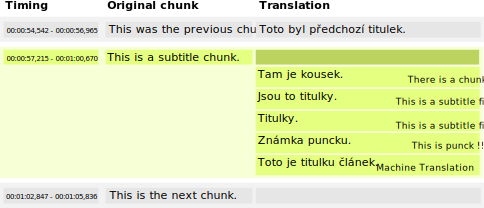
\includegraphics{./figures/current_strucutre.pdf}
\end{center}
\caption{Current scheme of the work with translation memory.}\label{fig:new_scheme}
\end{figure}

We agreed on the shared classes that all parts of the project should use. We more or less adopted the design of the classes from the core and started to use them in the whole project. This step required to re-implement some Scala classes in Java and to drop code that was already done in the User Space and the client. The design of the classes was almost the same as the final shared class design.

From a later point of view, it appears to be an important decision to agree on the shared classes, which made the cooperation between the modules easier and less verbose.


\subsubsection{GUI layout}

We started the work on the project with the new design soon, which lead to a period of struggles with technologies. It took us almost two months to have the first running version of the application.

The very first version of the application was a page where it was only possible to upload a subtitle file and to do the translation, without any possibility to load an already saved subtitle document or download the result of the translation, without any sessions or users; it was just a page where you edit the subtitles (which later became the Translation Workspace).


\subsubsection{External APIs}

At that time we used machine translation from the MyMemory service (which in fact wraps Google Translate), but there is a limited access per IP address and we soon began to reach the limit very frequently. It became obvious the we would have to change the source of machine translation. Based on that we decided to train our own Moses system. See Chapter~\ref{chap:moses} for details.

We also used an API providing IMDB.com information to receive information 
about movies but the movie meta data was not used in the evaluation the 
matches at that time. We had to switch to Freebase later because the IMDB service we used was discontinued.

\subsection{The Main Development Phase}

It is hard to define the main development phase which is covered in the 
following paragraphs. It corresponds to the period from the beginning of 
March when the important design changes were made (see previous 
Section~\ref{subsec:introducing_shared_classes}) to approximately the 
middle of August when adding new features was stopped (see the next 
Section~\ref{subsec:final_development}).

The section is divided to parts covering the issues we were dealing with 
and describes what we did in each area in those approximately five and 
half months.

\subsubsection{OpenID}
\label{subsubsec:openid}

Although we wanted to implement OpenID support from the very beginning, 
we started with it approximately in May. We found the two most frequently 
used Java libraries for OpenID and tried them. Those were \emph{JOpenID} 
and \emph{openid4java}.

\emph{JOpenID} seemed to be easier to use and also was much smaller as a 
dependency; on the other hand, when we ran into some problems with using 
it, we found out that \emph{openid4java} is much more frequently 
discussed on the \emph{StackOverflow.com} forum and that there is a 
bigger chance that we would be able to find some advice for potential 
problems. 

However, as discussed in \ref{us:openid}, \emph{openid4java} is easier to implement, so we used that, even for its biggest shortcoming -- users are not able to set their own OpenID provider.

The support for OpenID was finished in July, the parser for the authentication data from Seznam was added at the beginning of August.

\subsubsection{Chunk Splitting}

An interesting issue, also from the linguistic view, we had to solve was to find the best way of splitting the subtitle items into chunks. As opposed to the classical way of simply splitting documents into sentences, we had several possible ways of doing the splitting because of the nature of subtitle files.

We talk about chunk splitting more in chapter~\ref{os:sentence_splitting}.

We then realized that it is important that the splitting the same when importing subtitles into the database and when processing the user subtitles (as discussed in~\ref{os:guiparsing}), so we made it a shared class.

\subsubsection{Logging GUI}

After a while we found out that logging GUI errors is as important as logging userspace and core errors. We describe the GUI logging in section~\ref{gui:logging}; we first had a temporary debugging console, we switched it to remote logging mechanism at the beginning of August.

\subsubsection{Implementing the RPCs}

From the start, it was obvious to us that we want to use a well-established method to implement the Remote Procedure Calls.
We noted in the specification that we would probably use JSON for the message serialization.
Fortunately, GWT does provide a ready-to-use Remote Service implementation, which is described in bigger detail in chapter~\ref{sec:rpc:rpc}. GWT,  as a matter of fact, does actually serialize the messages to JSON internally.


\subsubsection{Sending Translation Results}

What we have been almost continually changing was the way the results are requested and then sent back by User Space. The discussion is described in greater detail in Section~\ref{sec:rpc:discussion_sending_results}.

\subsubsection{User Management}

At the very beginning the GUI was basically only the translation workspace. It was possible to translate a subtitle file in the application, the changes were reflected in the database, however it was not possible to get them in the application when the web application was reloaded or to export the subtitles.

We considered the user management to be just a minor technical issue. However, to enable to reach the intended architecture of the User Space -- mostly that most of the calls should be resolved in the Session objects -- we introduced a simple fake login in April (you could log as any user using password "guest").

We started to implement the OpenID login support in May (see Section~\ref{subsubsec:openid}). When we met some technical difficulties, we decided to implement our own registration and login first.

For more information about user management, see part \ref{us:usermanag}.

\subsubsection{GUI Look and Feel}

The design of the GUI was driven by the intentions of effectiveness, while retaining a smooth look at the same time. The effectiveness was achieved by stressing the keyboard-oriented control of the components and simplicity of their layout. The need of a pleasant visual feeling was the reason for using the Twitter Bootstrap design, bringing a user friendly feeling of the application at a very little cost.

\begin{figure}
\begin{center}
\includegraphics[scale=0.5]{figures/old_screenshot.png}
\end{center}
\caption{Design of the Translation Workspace before starting to use the Twitter Bootstrap}
\label{fig:before_bootstrap}
\end{figure}

\subsubsection{GUI Pages}

We started having one page only, the Translation Workspace, which was sufficient for development of the application for several months. Later we added the Document  Creator page as the default one, which replaced itself by the Translation Workspace once a document was created, and this was sufficient for some more time. However, we eventually could not avoid adding more pages and the need to explicitly handle multiple pages became obvious.

This lead to some problems, because GWT cannot easily handle more pages, which genuinely surprised us.

We describe the problems and their solutions in the chapter~\ref{gui:gwt}


\subsubsection{Handling Parsing Errors}

% At first, the subtitle files were expected to be in the correct format -- no explicit checks were performed and if an error was encountered, the file was rejected.
% The SrtTime class was then added 

We found that since many subtitle files are partly or fully generated by users, and probably also because the SRT format has no official specification, errors in the files are very common. Rejecting even the files with only minor errors (such as a surplus or missing newline, or an incorrect time format which we check thoroughly) showed to be unnecessarily strict, as typically most of the file is correct and the number of errors is small.

We decided to introduce heuristics to decide whether to reject the whole file: if the number of recoverable errors is lower than 10, the erroneous parts are skipped and the rest of the file is parsed.


% However, this lead to also rejecting
% We were improving the situation gradually, eventually creating a new exception class, InvalidDocumentFormatException, which is thrown by the parser, with a 
% Also, as a preliminary check, we refuse any file which is larger than 500 kB. We introduced this check because it is very fast and efficient.

\subsubsection{Offline Mode}
\label{ip:subsubsec:offline}

At first, our intention was to make the whole application able to run offline. However, it was not a priority and was not even part of the official specification.

When we tried the HTML5 Local Storage, though, the offline mode seemed to be actually easy to implement using this technology, while the support for it is good across web browsers.

The Offline mode is described in bigger detail in Chapter~\ref{gui:offlinemode}


\subsubsection{Subgestboxes}

One of the most important features of the application's user interface is the behavior of the actual translation workspace, particularly the text-boxes where user writes their translations and which provide the pop-up suggestions from the translation memory. Since the functional requirements for these boxes were gradually refined throughout the development process, their implementation also underwent several stages of evolution. However, their class\' name, {\tt SubgestBox}, remained from the early stages, implying the idea of a box offering suggestions for subtitles.

Since the GWT pre-implemented {\tt SuggestBox} did not meet our requirements we had to find our own solution using HTML IFrames and GWT {\tt RichTextArea}. It provided all the functionality we have requested, but there was a significant performance problem -- the browser often became irresponsive when loading hundreds of them. We solved this by distinguishing so-called ``fake'' and ``real'' {\tt SubgestBoxes}; it is described in bigger detail in Chapter~\ref{gui:subgest}.


%We don't want to repeat GUI chapter
%The {\tt RichTextArea}, being based on the IFrame HTML element, provided all the functionality we have requested (although some of it is not as simply accessible as we expected), but there was yet another problem with it. Having one IFrame for each chunk on the page, i.e. hundreds of them for an average movie, turned out to be quite a significant performance problem -- the browser often became irresponsive. In the end, we have solved this issue by distinguishing so-called ``fake'' and ``real'' {\tt SubgestBoxes}; the former being simple {\tt TextAreas} and displayed by default in the translation workspace, on focus transforming into the latter, the real IFrame-based {\tt SubgestBoxes} with all the functionality. This also required special approach in CSS styling.

Another issues as focus handling, automatic scrolling, dealing with endlines (see Table~\ref{implprocess:RichTextAreaNewlines} for details) and automatic resizing had to be solved in order to make the Translation Workspace more user-friendly.

\begin{table}[h]
\smaller
\begin{center}
\begin{tabular}{|l|l|l|}
\hline
\textbf{Browser} & \textbf{getText()}             & \textbf{getHTML()} \\
\hline
Firefox & \verb=first linesecond line= & \verb=first line<br>second line<br><br>= \\
\hline
Chrome  & \verb=first line=            & \verb=<div>first line</div><div>second line</div><div><br></div>= \\
        & \verb=second line=           & \\ 
\hline
Safari  & \verb=first line=            & \verb=first line<div>second line</div><div><br></div>= \\
        & \verb=second line=           & \\
\hline
IE9     & \verb=first line=            & \verb=<p>first line</p><p>second line</p><p>&nbsp;</p>= \\
        & \verb=second line=           & \\
\hline
Opera   & \verb=first linesecond line= & \verb=<p>first line</p><p>second= line</p><p><br></p> \\
\hline
\end{tabular}
\end{center}
\caption{Table capturing different handling of newlines across browsers, showing the return values of the RichTextArea's getText() and getHTML() methods. In all the cases, the text entered was ``first line[enter pressed]second line[enter pressed]''.}\label{implprocess:RichTextAreaNewlines}
\end{table}

\subsubsection{Subtitles Export}

When implementing the subtitles export feature, we encountered an unexpected issue:
GWT cannot create a new file, neither on server (because it is all JavaScript) nor on the user's computer (because of security restrictions).

We found several possible solutions:

\begin{itemize}

\item export the subtitles into a text area
\begin{itemize}
\item the easiest to implement
\item not what a user expects
\item not easy to use for the user
\end{itemize}

\item send the exported subtitles to user's e-mail address
\begin{itemize}
\item quite easy to implement because we already have implemented the e-mail sending
\item might be useful for some users
\item not what a user expects
\item can be hard to use for the user
\item might be added as a special feature but should not be the only or primary way
\end{itemize}

\item create a temporary file on the server and offer a download link to the user
\begin{itemize}
\item expected behavior from the user (file download using the browser)
\item reasonably reliable
\item reasonably easy to implement
\item should handle access rights in Jetty which is an added complication
\item creating temporary files is not very clean
\end{itemize}

\item create a new servlet (using JSP) for downloading the file
\begin{itemize}
\item expected behavior from the user (file download using the browser)
\item probably the cleanest possible solution
\item we were afraid that it would be too much extra work, but we realized that it was not so difficult
\end{itemize}

\end{itemize}

Eventually, we decided for the last option as the best one; therefore, the User Space actually consists of two servlets, one to handle RPCs and another for file download.

\subsubsection{Chunks saving/loading}

We originally decided that the subtitle file will be parsed in the GUI, 
to avoid unnecessary sending of the data from GUI to User Space and then back from User Space to GUI; parsing the file in User Space would also cause unnecessary load on the server.

Although we wanted to make everything as parallel as possible, we found out that we have to save all the chunks immediately after parsing so that they do not get lost; therefore, requesting the translation suggestions is only done after that, even though this means that the translation suggestions start arriving a little later.

To also enable editing the files, the Translation Workspace became the only page that has two constructors -- one receiving the text of a subtitle file to parse, and the other getting an already parsed document from the database.

\subsubsection{Finalizing and training the translation pair rankers}

Although the candidate search was started early in the development process, the ranking of candidates was not completed until the main development phase. Since we base the ranking on combining various scores with weights, it is necessary to estimate these weights from data. In order to produce the annotated data for this, all other parts of the system had to be fully functional. Because of this, we could finalize the ranking and train the ranking models only later in the main development phase.

\subsubsection{Machine translation}
Altough machine translation with Moses was thought to be just a nice possibility to have and weren't given too much attention initially, at the end we were very surprised with how accurate it is on our data (seeing it being more successful than Google Translate was a \emph{very} gratifying moment) and how quick we managed to finally get it.

The only problematic part was fitting both our application and Moses on the same small virtual machine we were given for this project. However, when we deleted all unnecessary data from the disk and ran with only the binarized models, we were able to run it fine (even when we have only about 1 GB of free disk space, but it seems to be enough for Jetty).

\subsection{Final Development}
\label{subsec:final_development}

We left many issues which we considered to be only minor and technical
to the end of the development process;
some of these issues were eventually found to constitute intensive work.

We set the Feature Freeze to the 12$^\mathrm{th}$ August, 12 p.m.
After the Feature Freeze, no new features were added to the project, and 
we started an intensive review of already existing code, debugging, and 
working on the documentation. After the feature freeze, we improved 
stability of the application and its responsiveness. 


\section{Evaluating the Development Process}

\subsection{Technologies}
One of the crucial decision for the project was the choice of technologies. Most of the technologies we used -- Maven, Scala, Hibernate, GWT -- were new to some of us and we also had not much experience with the other. Combining these technologies together was a difficult task and would probably even be for an experienced Java developer. Generally, because we were not too very familiar with the technologies, we spent most of the time solving technical issues. There are numerous research challenges, mostly in the fuzzy matching part, which had to remain untouched due to that. Nevertheless, it is doubtful if this was caused only by technical difficulty or by paying too much attention to less important technical tasks.


A bottleneck of the development process was also that not all of us were familiar with all of the technologies. It happened several times that somebody could not continue developing a particular part of the project and had to wait for another team member to fix the issue.

On the other hand, our choice of technologies appeared to also be good since it saved a significant amount of work for us due to the possibility to share an implementation of a class. Using the Scala language for the core also made the parallelization much easier.

\subsection{Structure}
Although we spent a long time on discussions of how the structure of the project would look like, we did not avoid a radical change of the design of the application a few months after the project started. Nearly the whole User Space code had to be dropped and it was also necessary to totally remake the client components existing so far.

\subsection{Efficiency, communication}
During the whole time we had the problem that our development process was not as effective as we would imagine and it was also difficult to find a suitable communication platform. Although we saw each other often to discuss the project issues and had regular meetings, a working online communication played a crucial role for us.

As a very first communication channel, we established a mailing list at Google groups. All the notifications and comments from Github were redirected to that mailing list, as well as results of Jenkins builds. Soon, we started to receive dozens of FilmTit email every day and it started to be quite difficult the follow the conversations and find items in the conversation history.

Because of this, we tried to use PiratenPad\footnote{\url{http://www.piratenpad.de/}}. It is free a web-based collaborative real-time editor, allowing authors to simultaneously edit a text document, and see all of the participants\' edits in real-time, with the ability to display each author's text in their own color. There is also a chat box in the sidebar to allow meta communication. The service is run by the German Pirate Party. We tried to use the tool to gather personal plans and ``todos'', bug reports, etc. After some time, the pads became messy and the mailing group became the main communication channel again. We were also solving many issues bilaterally using various instant messaging systems.

In July, %when the most intensive work on project started,
we launched a Skype group chat. It effectively replaced the personal meetings, which was much sought after as usually several members were out of Prague at a time, but fortunately, they typically had an Internet connection.
It also helped to solve many issues instantly and efficiently.
However, it has a same disadvantage as email conversation -- it is difficult to easily find facts in the history -- but now with hundreds of messages every day to make things worse.
Fortunately, because almost every time there were at least some team members online, it was always possible to ask for a summary of the previous discussions and we managed to keep all the team members informed about everything important.

%Mid-August, however, there was a decline in using the Skype group -- we found out that when all of the project members were online and the work on the project could have been expected to be very intensive, it often actually happened that very little work was done since most of the time was spent on discussions through Skype.
%Another issue was that some members tended to use the conference simply for chatting about non-related matters, %including me of course --R
%which later made it even harder or nearly impossible for the others to find important messages in the history.
%We then started to send the most important messages through the e-mail conference again and, eventually, we mostly switched back to it.


\section{Work Distribution}

\subsection*{Karel Bílek}

\begin{itemize}
	\item implementation of the VLC playback and java applet
	\item processing the OpenSubtitles.org data
	\item preparing and optimization of the Moses system to our use
	\item initialization of Jetty webserver
\end{itemize}

\subsection*{Josef Čech}

\begin{itemize}
	\item development of the User Space
\end{itemize}

\subsection*{Joachim Daiber}

\begin{itemize}
	\item design and implementation of the Core Translation Memory, searching, ranking, merging, import, indexing, media source retrieval, etc.
	\item evaluation of database systems
	\item parts of the GUI layout, stylesheet and general fixes in GUI
	\item set up continuous build system, initial Maven project, configuration management
\end{itemize}



\subsection*{Jindřich Libovický}

\begin{itemize}
	\item early processing of the opensubtitles.org data
	\item design and implementation of the User Space
\end{itemize}


\subsection*{Rudolf Rosa}

\begin{itemize}
	\item development of many functions of GUI (login, Offline Mode, pages, dialogs, settings etc.)
	\item Remote Procedure Calls and their GUI implementation
\end{itemize}


\subsection*{Jan Václ}

\begin{itemize}
	\item development of the GUI (structure, visual appearance and experience, Translation Workspace)
\end{itemize}


\section{Possible Future Development}

There are many issues to be improved, mostly in the graphical interface. It would probably be possible to add new features forever. A newer version would likely include support for more language pairs.

We would like to let the project run for some time and wait if it would find its community of users. If it would reach some success among the user, it could provide much interesting data -- mostly about preferences of the users about which translation suggestions are useful for them. Such information could be useful for developing new fuzzy matching techniques including some research challenges, such as finding matches to only a part of a sentence. Success among users would also mean a growing source of well structured data for statistical machine translation.



\part{Manuals}

\chapter{Technical Manual}

\section{Tasks}



\subsection{Importing data}

\subsubsection{Alignment}


\subsubsection{Import}

\lstset{numbers=none, language=bash, caption={Settings for the Data Import}}
\begin{lstlisting}
$ java ...
\end{lstlisting}




\section{Configuration}

The configuration for the server is contained in the file \verb#configuration.xml#, which has to be specified on startup.

In this section, we will give a brief overview over the properties specified in the configuration file and its default values.

\subsection{General settings}
L1 and L2 specify the ISO 639-1 codes of the source and target languages used in the translation memory.
\lstset{numbers=none, language=XML, caption={Languages}}
\begin{lstlisting}
<l1>en</l1>
<l2>cs</l2>
\end{lstlisting}

\subsection{Database}

The database connection must be specified as a valid JDBC connector. By default, the DBMS is the local Postgres database \verb#filmtit# with default username and password.

\lstset{numbers=none, language=XML, caption={Database connection}}
\begin{lstlisting}
<database>
    <connector>jdbc:postgresql://localhost/filmtit</connector>
    <user>postgres</user>
    <password>postgres</password>
</database>
\end{lstlisting}

\subsection{Text processing models}

For various text processing tasks within the translation memory, 
it is necessary to specify a number of model files.

The system will search for the models in the folder \verb#model_path#.
\lstset{numbers=none, language=XML, caption={Model path}}
\begin{lstlisting}
<model_path>models/</model_path>
\end{lstlisting}

OpenNLP Maximum Entropy tokenizer models are specified in the \verb#tokenizers# section. If for a specific language, no tokenizer model is specified, the translation memory will use the default OpenNLP WhitespaceTokenizer.
\lstset{numbers=none, language=XML, caption={Tokenizers}, }
\begin{lstlisting}
<tokenizers>
    <tokenizer language="en">en/token.bin</tokenizer>
    <tokenizer language="cs">cs/token.bin</tokenizer>
</tokenizers>
\end{lstlisting}

OpenNLP Maximum Entropy models for Named Entity Recognition are specified in the \verb#ner_models# section. Each \verb#ner_model# specifies a language (ISO 639-1 code) and the type of Entity that it recognizes. Currently, only Person, Place and Organization are used. If fewer models are specified, only the specified models will be used.

\lstset{numbers=none, language=XML, caption={Models for Named Entity Recognition}}
\begin{lstlisting}
<ner_models>
    <!-- English -->
    <ner_model language="en" type="Person">en/ner-person.bin</ner_model>
    <ner_model language="en" type="Place">en/ner-place.bin</ner_model>
    <ner_model language="en" type="Organization">en/ner-organization.bin</ner_model>

    <!-- Czech -->
    <ner_model language="cs" type="Person">cs/ner-person.bin</ner_model>
    <ner_model language="cs" type="Place">cs/ner-place.bin</ner_model>
    <ner_model language="cs" type="Organization">cs/ner-organization.bin</ner_model>
</ner_models>
\end{lstlisting}

\subsection{Data Import}
%TODO section?
For the data import as described in section~\ref{sec:dataimport}, several files have to be specified.

\begin{itemize}
        \item \verb#subtitles_folder# -- the folder containing the subtitle files for the initial import
        \item \verb#data_folder# -- the folder the results of the alignment (see section~\ref{sec:dataimport})
        \item \verb#file_mediasource_mapping# -- a CSV file that describes the source (movie or TV show) of the  subtitle files
        \item \verb#batch_size# -- the number of subtitle files that should be processed at the same time. A higher number will increase the memory consumption of the import process.
        \item \verb#imdb_cache# -- the location of a cache file for the movie data queried from IMDB for each subtitle file
        
        \item \verb#heldout# -- specifies a portion of the data that will be left out of the import for tuning purposes
\end{itemize}


\lstset{numbers=none, language=XML, caption={Settings for the Data Import}}
\begin{lstlisting}
<import>

    <subtitles_folder>/filmtit/data/export/files/</subtitles_folder>

    <data_folder>/filmtit/data/aligned/</data_folder>
    <file_mediasource_mapping>/filmtit/data/files/export_final.txt</file_mediasource_mapping>
    <batch_size>100</batch_size>
    <imdb_cache>/filmtit/data/imdb_cache</imdb_cache>

    <heldout>
        <size>0.02</size>
        <path>/tmp/heldout.csv</path>
    </heldout>

</import>
\end{lstlisting}


\subsection{Module-Specific Options}

\subsubsection{Core TM}

The module-specific options for the Core TM are mostly related to performance.

\begin{itemize}
        \item \verb#max_number_of_concurrent_searchers# -- specifies the maximum number of searchers that will be created concurrently. By default, 5 searchers will be created and requests will be scheduled among them.
        \item \verb#searcher_timeout# -- specifies the maximum time the scheduler will wait for a searcher to respond. If the time is exceeded, the scheduler will retry a different searcher.
\end{itemize}

\lstset{numbers=none, language=XML, caption={Settings for the Core TM}}
\begin{lstlisting}
<core>
    <max_number_of_concurrent_searchers>5</max_number_of_concurrent_searchers>
    <searcher_timeout>60</searcher_timeout> <!--in seconds-->
</core>
\end{lstlisting}


\subsubsection{Userspace}

\lstset{numbers=none, language=XML, caption={Settings for the Userspace}}
\begin{lstlisting}
<userspace>
    <session_timeout_limit>3600000</session_timeout_limit>
    <server_address>http://ufallab.ms.mff.cuni.cz:12480</server_address>
</userspace>
\end{lstlisting}



\chapter{User Manual}
\label{chap:users_manual}




\end{document}
